\chapter{Thực nghiệm}
\ifpdf
    \graphicspath{{Chapter5/Chapter5Figs/PNG/}{Chapter5/Chapter5Figs/PDF/}{Chapter5/Chapter5Figs/}}
\else
    \graphicspath{{Chapter5/Chapter5Figs/EPS/}{Chapter5/Chapter5Figs/}}
\fi
\label{chap_5}

\begin{quote}
\textit{Để đánh giá hiệu năng của các đặc trưng và mô hình kết hợp thông tin màu-độ sâu đã trình bày, trong chương này khóa luận tiến hành thí nghiệm trên nhiều tập dữ liệu với tính chất khác nhau như: dữ liệu thuần độ sâu, dữ liệu gồm cả màu và độ sâu, dữ liệu cho bài toán từ nhận dạng từ cử chỉ-hành động đơn đến cả chuỗi hành động liên tục theo thời gian. Thực nghiệm cho thấy mô hình trích chọn-biểu diễn-kết hợp các đặc trưng từ dữ liệu RGB-D, được đề xuất trong khóa luận, đã đem lại những kết quả rất khích lệ, cụ thể là đạt độ chính xác cao hơn so với các nghiên cứu state-of-the-art trên nhiều tập dữ liệu hành động khác nhau.}\\
\textit{Lưu ý tất cả các tập dữ liệu cử chỉ-hành động được sử dụng trong khóa luận đều là dữ liệu chuẩn quốc tế do Microsoft tạo  và công khai sử dụng cho mục đích nghiên cứu.}
\end{quote}

\section{Nhận dạng hành động người trên tập MSRAction3D\cite{Wu_LOP2012}}
\label{sec_action3d_exp}
Trong thí nghiệm này, khóa luận tiến hành đánh giá khả năng biểu diễn của đặc trưng 3DS-HONV trên dữ liệu độ sâu, cụ thể là xét trong ngữ cảnh nhận dạng hành động người trên video. Qua việc phân tích các kết quả đạt được, khóa luận đề xuất một giải pháp tăng cường thông tin cho 3DS-HONV bằng cách kết hợp đặc trưng này với đặc trưng HOF trích chọn trên chuỗi ảnh độ sâu (gọi là DHOF). Bên cạnh đó, để tăng cường khả năng biểu diễn và đảm bảo tính bất biến của các đặc trưng rút trích được với các phép dịch, biến đổi tỷ lệ, thuật toán tạo codebook SC (trình bày trong chương \ref{sec_sparse_code}) sẽ được áp dụng trên từng khối thể tích con (sub-volume) của các chuỗi hành động. Trong các phần dưới đây, khóa luận trước tiên giới thiệu về tập dữ liệu, cách thiết lập thí nghiệm và các tham số cài đặt, cuối cùng là kết quả đạt được khi sử dụng các đặc trưng 3DS-HONV, phiên bản kết hợp 3DSHONV-DHOF, và dạng biểu diễn thưa của các đặc trưng này sử dụng SC. 
\subsection{Giới thiệu tập dữ liệu}
\begin{figure}
\centering
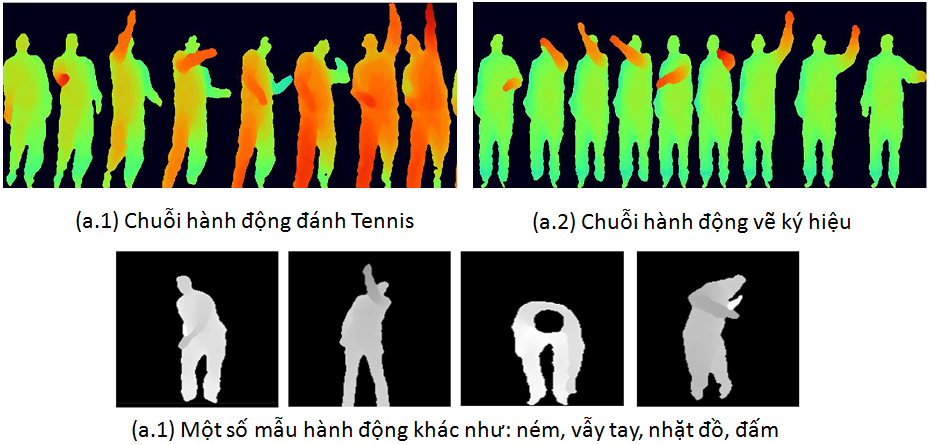
\includegraphics[scale=0.6]{action3d_samples.png}
\caption{Minh họa một số mẫu hành động trong tập MSRAction3D: (a.1-2) Chuỗi ảnh độ sâu được chuyển sang màu RGB để hiển thị và mô tả 2 hành động, (b) Một số mẫu dữ liệu khác.\cite{Wu_LOP2012}}
\label{fig_action3d}
\end{figure}
MSRAction3D là tập dữ liệu hành động thu được từ camera độ sâu. Tập dữ liệu gồm tổng cộng 20 hành động sau: "\textit{high arm wave, horizontal arm wave, hammer, hand catch, forward punch, high throw, draw x, draw tick , draw circle, hand clap, two hand wave, side-boxing, bend, forward kick, side kick, jogging, tennis swing, tennis serve, golf swing, pick up \& throw}" \cite{Wu_LOP2012}. Các hành động này được thực hiện bởi 10 chủ thể, mỗi người 3 lần. Ngoài thông tin độ sâu, tập dữ liệu này còn cung cấp thêm thông tin về khung xương của người tương ứng với từng mẫu dữ liệu. Về tổng thể, tập dữ liệu MSRAction3D gồm 23797 frame ảnh độ sâu và 402 mẫu hành động. Một số mẫu dữ liệu trong MSRAction3D được minh họa trong hình \ref{fig_action3d}.

\subsubsection{Thách thức của tập dữ liệu:} Sự tách biệt giữa các lớp hành động là tương đối nhỏ, ví dụ như: hành động ném và đánh tennis,... Bên cạnh đó, việc dùng thông tin khung xương được cung cấp cũng xảy ra rất nhiều nhiễu và không chính xác.
\subsection{Cách thiết lập thí nghiệm}
\begin{figure}
\centering
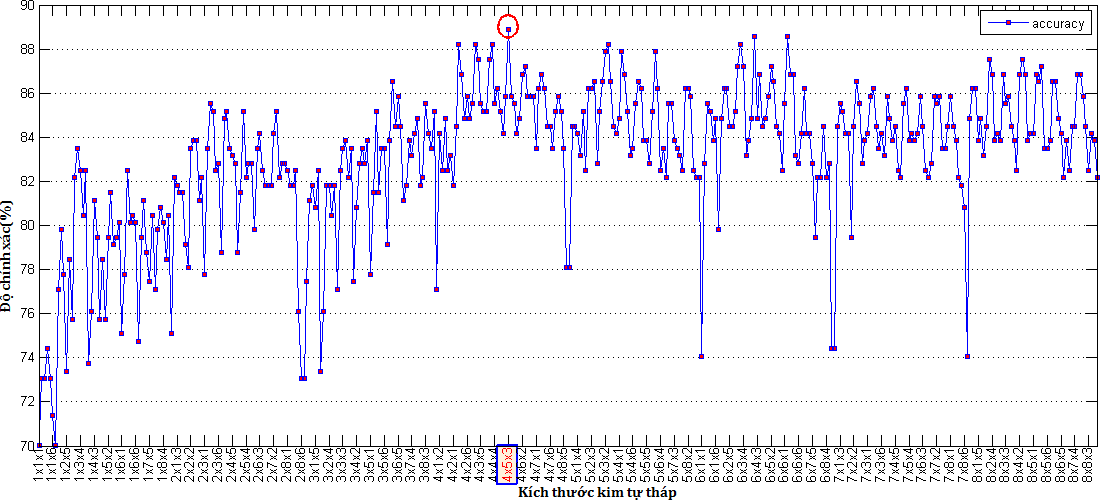
\includegraphics[scale=0.55]{action3d_params_tunes.png}
\caption{Kết quả phân lớp trên tập dữ liệu MSRAction3D với $8\times 8\times 6$ trường hợp thay đổi kích thước kim tự tháp không-thời gian.}
\label{fig_action3d_params_tune}
\end{figure}

	\begin{algorithm}
	\newalgname{Giải thuật}
	\caption{Giải thuật rút trích-biểu diễn đặc trưng \& phân lớp trên tập dữ liệu MSR-Gesture3D và Action3D}
	\label{alg_gesture_action3d}
	\begin{algorithmic}
	\renewcommand{\algorithmicrequire}{\textbf{Đầu vào:}}
	\renewcommand{\algorithmicensure}{\textbf{Đầu ra:}}
	\algnewcommand\algorithmicoperation{\textbf{Thao tác:}}
	\algnewcommand\Operation{\item[\algorithmicoperation]}
	
	\Require 
	\State M mẫu video độ sâu dùng để huấn luyện \(S^{tr} = \{S^{tr}_1,...,S^{tr}_M\}\)	
	\State Tập vector đặc trưng rút từ các mẫu huấn luyện: \(H^{tr} = \{H^{tr}_1,h^{tr}_2,...,h^{tr}_M\}\) (tính từ tầng huấn luyện)
	\State Tập Codebook đã học: \(B\) (được tính từ bước huấn luyện).
	\State N mẫu test (video độ sâu): $S^{te} = \{S^{te}_1,...,S^{te}_N\}$
	
	\Ensure 
	\State Kết quả nhận dạng: \textit{Lóp hành động ($class$)}
	
	\Operation \\	
	\begin{enumerate}		
		\item Tiền xử lý: Loại nhiễu sử dụng bộ lọc song phương (\textit{bilateral filter} \cite{camplani_jbf}): 
			\begin{equation}
			BF[\hat D(p)] = \frac{1}{{W_p}} {\sum\limits_{q \in {\Omega _p}} G_{\sigma_s} f(p,q) \hspace{0.05in}G_{\sigma_r} \left( {\left\| {D(p) - D(q)} \right\|} \right) \hspace{0.05in}D_q}
			\end{equation}
		\item Khởi tạo: $class = [\hspace{0.05in}]$
		\For{$i=1;i\le N;i++$}		
			\State Chia $S^{te}_i$ thành $n_c = n_x\times n_y\times n_t$ khối con (cells) tuần tự theo các trục $x,y,t$			
			\State Rút và kết hợp đặc trưng \textbf{3DS-HONV}, \textbf{DHOF} để biểu diễn cho từng cells: \(h^{te}_{j=1..n_c}\)
			\State Tại mỗi cell $c_{j=1..n_c}$, tính biểu diễn thưa $X_j$ của đặc trưng \textbf{3DSHONV-DHOF} dựa trên codebook $B_{c_j}$, sử dụng thuật toán SC\cite{Andrew_sparse_coding}
			\begin{equation}
			\begin{array}{l}
			\textbf{Codebook:}\hspace{0.1in} < B,U > = \mathop {\min }\limits_{B,U} \left\| {H - BU} \right\|_2^2 + \lambda {\left\| U \right\|_1} s.t.\hspace{0.1in}\forall k,{\left\| {{u_k}} \right\|_0} \le T \\
			\hspace{1.5in} \hat H^{tr} = U \\
			 \textbf{Reconstruct:}\\
			 \hspace{1in} {x_{c_i}} = \arg \mathop {\min }\limits_{{x_{c_i}}} \{ \left\| {{h_{c_i}} - B_{c_i}{u_{c_i}}} \right\|_2^2\} \hspace{0.15in} s.t.{\left\| {{x_{c_i}}} \right\|_0} \le T
			 \end{array}
			\end{equation}
%			\begin{equation}
%			\begin{array}{l}
%			 \textbf{Codebook:}\hspace{0.1in} < B,A,U >  = \arg \mathop {\min }\limits_{B,A,U} \left\| {H^{tr} - BU} \right\|_2^2\\
%			 \hspace{1.8in} + \alpha \left\| {Q - AU} \right\|_2^2 \hspace{0.15in} s.t.\hspace{0.1in}\forall k,{\left\| {{u_k}} \right\|_0} \le T \\ \\			 			 
%%			 \textbf{Codebook:}\hspace{0.1in} < B,A,X} >  = \arg \mathop {\min }\limits_{B,A,X} \left\| {{h^{te}_j} - BX \right\|_2^2
%%			 \hspace{0.8in} + \alpha \left\| {Q - AX_j} \right\|_2^2 \hspace{0.15in} s.t.\hspace{0.1in}\forall k,{\left\| {{x_k}} \right\|_0} \le T \\
%			 \textbf{Reconstruct:}\hspace{0.1in} \hat H^{tr} = AU \\ \\
%			 \hspace{1in} {x_{c_i}} = \arg \mathop {\min }\limits_{{x_{c_i}}} \{ \left\| {{h_{c_i}} - B_{c_i}{u_{c_i}}} \right\|_2^2\} \hspace{0.15in} s.t.{\left\| {{x_{c_i}}} \right\|_0} \le T
%			\end{array}
%			\end{equation}
			\State Tính hist $h_i^{te} = \mathop  \odot \limits_{j = 1..{n_c}} u_{c_j}^{te}$ để biểu diễn cho $S_i$ (\gls{acr_concate} là toán tử nối vector)
			\State \textbf{Phân lớp}: $tmp\_class = svm\_classify(h_i^{te}, \hat H^{tr})$ 
			\State $class = [class\hspace{0.1in} tmp\_class]$
		\EndFor \\
		\Return \textit{class}	
	\end{enumerate}		
	\end{algorithmic}
\textit{	Chú thích: \gls{acr_st} là thỏa điều kiện, \gls{acr_hist} là histogram.}
	\end{algorithm}

Tổng quan về quy trình thiết lập thí nghiệm cho tập dữ liệu MSRAction3D (và cả tập MSRGesture3D) được trình bày qua giải thuật \ref{alg_gesture_action3d}. Cần làm rõ thêm là do tính chất của tập dữ liệu có rất nhiều nhiễu và bài báo \cite{Omar_HON4D} cũng đã chứng minh các bộ dò điểm trong yếu sẽ không hoạt động tốt trên tập dữ liệu này, vì vậy khóa luận sẽ thực hiện chiến lược lấy mẫu mật độ cao (\textit{dense sampling}) trên tất cả các video độ sâu.\\
Theo đó, để đạt được hiệu suất nhận dạng tốt nhất trên mô hình thuật toán đã đề xuất, khóa luận tiến hành việc tìm ra các tham số tối ưu thông qua quá trình "kiểm chứng chéo" (\textit{cross-validation}). Kết quả thu được là các tham số tối ưu được thiết lập như sau:
\begin{itemize}
	\item Bộ tham số kích thước kim tự tháp không-thời gian (\textit{spatial-temporal pyramid}) phân chia trên mỗi chuỗi hành động: $n_x=4$, $n_y=5$, $n_t=3$. Hình \ref{fig_action3d_params_tune} minh họa các kết quả phân lớp thu được qua quá trình tối ưu tham số trên lưới tìm kiếm (\textit{grid search}); kích thước lưới tìm kiếm được cài đặt là $n_x=[1:8],n_y=[1:8],n_t=[1:6]$. Như vậy có tổng cộng $8\times8\times6=384$ trường hợp.
	\item Cần lưu ý rằng quá trình tạo codebook trong khóa luận được tiền hành độc lập trên từng khối con (cell) trong kim tự tháp không-thời gian. Kích thước codebook tối ưu chọn được trong thí nghiệm là: 200 (\textit{từ}) cho mỗi cell.
	\item Số chiều của đặc trưng DHOF (đặc trưng HOF chuẩn \cite{Dalal_HOF} tính tại mỗi điểm trên ảnh độ sâu) là: 9 (bins)
	\item Số bin không-thời gian thiết lập cho đặc trưng 3DS-HONV là: $b_\theta = 5$, $b_\phi = 5$, $b_\psi = 6$
\end{itemize}
\textit{Như vậy, về cơ bản, tại mỗi cell số chiều của các vector đặc trưng lần lượt là: $150-bins$ \textbf{3DS-HONV}, $9-bins$ \textbf{DHOF}, $159-bins$\textbf{3DSHONV-DHOF}, $200-bins$ \textbf{3DSHONV-DHOF + SC}}. 

Thuật toán phân lớp được sử dụng trong thí nghiệm này và thí nghiệm trên tập MSRGesture3D là \textbf{SVM} phi tuyến, sử dụng kernel đa thức, chiến lược huấn luyện là \textit{one-vs-all}. Lưu ý, quy trình thiết lập thí nghiệm này được thực hiên giống với bài báo \cite{Omar_HON4D} để thuận tiện cho việc đánh giá và so sánh giữa các phương pháp. Cụ thể hơn, để tiến hành thí nghiệm, khóa luận thực hiện chia tập dữ liệu làm đôi, một nửa đầu (5 chủ thể hành động) dùng cho việc huấn luyện và nửa còn lại dùng cho mục đích đánh giá. 

	
\subsection{Kết quả thực nghiệm}
\begin{figure}
\centering
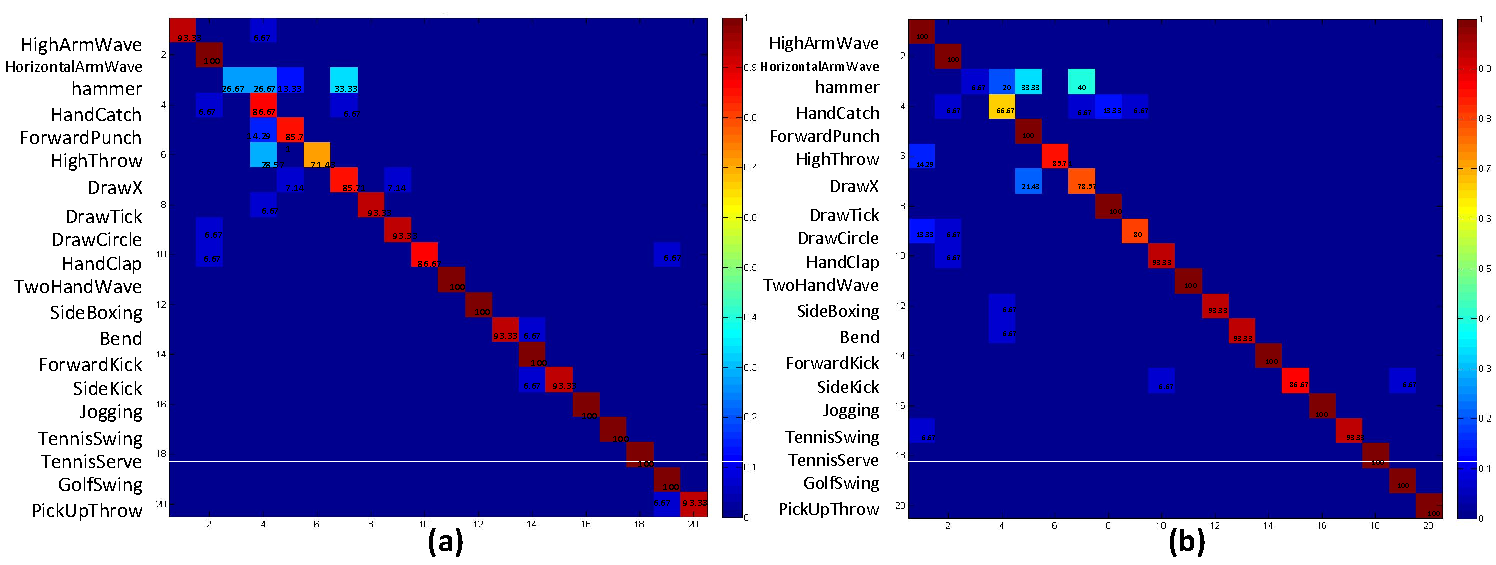
\includegraphics[scale=0.66]{action3d_both.pdf}
%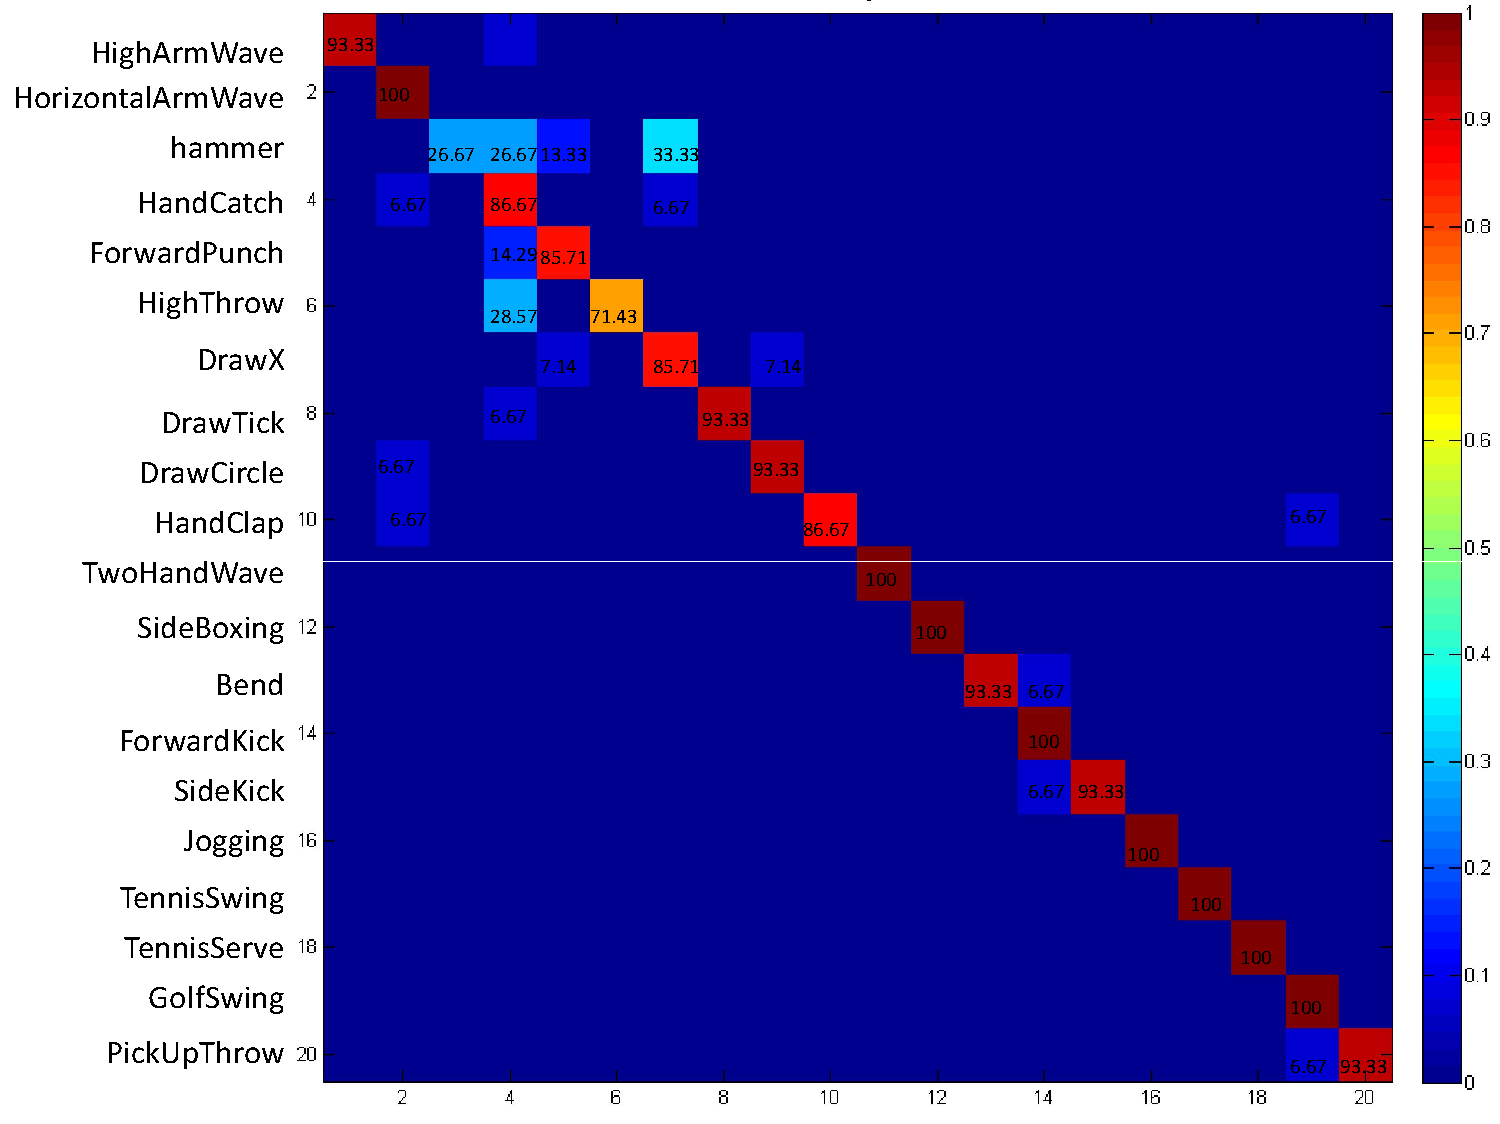
\includegraphics[scale=0.4]{aciton3d_honv_dhof.pdf}
\caption{Ma trận confusion trên tập dữ liệu MSRAction3D khi sử dụng phương pháp: (b)Đặc trưng kết hợp 3DSHONV-DHOF, (b)Đặc trưng 3DS-HONV}
\label{fig_action3d_both_conf}
\end{figure}	

\begin{figure}
\centering
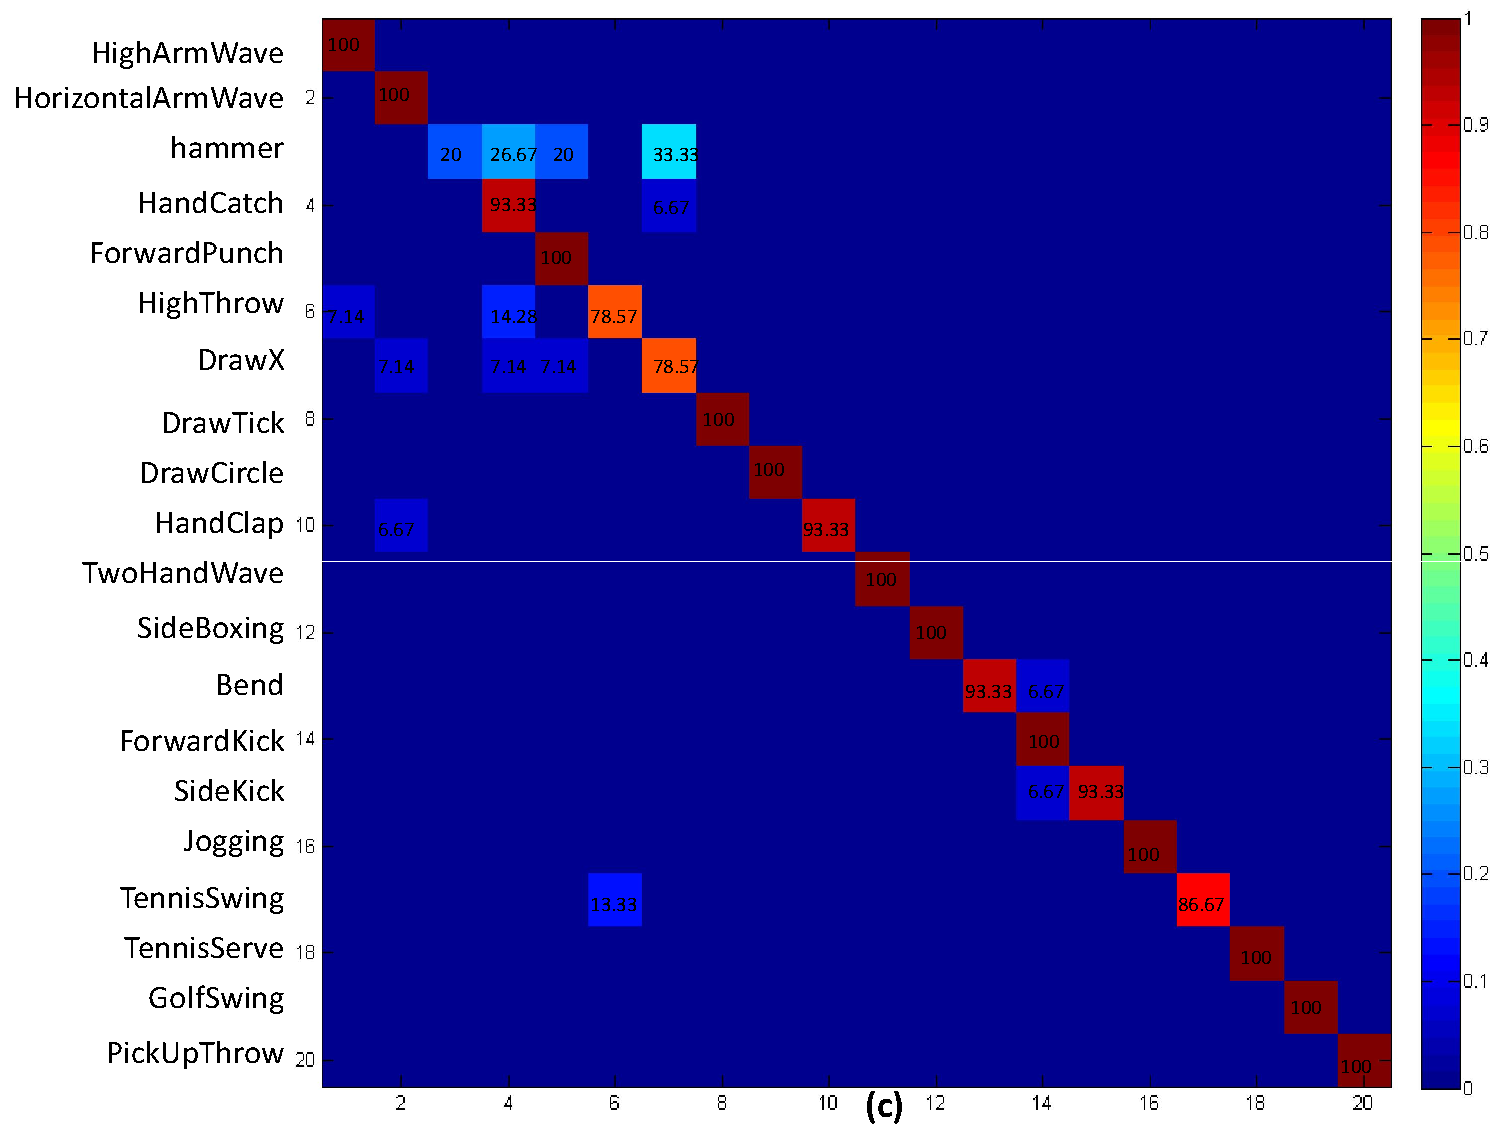
\includegraphics[scale=0.4]{action3d_lcksvd.pdf}
\caption{Ma trận confusion trên tập dữ liệu MSRAction3D khi sử dụng phương pháp biểu diễn thưa trên đặc trưng 3DSHONV-DHOF}
\label{fig_action3d_sparse_conf}
\end{figure}	

\begin{table}
	\caption{So sánh giữa các phương pháp đề xuất với các nghiên cứu trước trên tập MSR-Action3D}
	\centering 
	\begin{tabular}{l c}	
	\hline\hline
	\textbf{Phương pháp} & \textbf{Độ chính xác \%} \\	
	\hline\hline
	\textbf{3DSHONV-DHOF + sparse coding} & \textbf{91.92}\\ 
	\textbf{3DSHONV-DHOF (đề xuất)} &  \textbf{90.23}\\ 
	\textbf{3DSHONV (đề xuất}) & \textbf{88.89}\\
	\hline \hline
	Omar et al. \cite{Omar_HON4D} (HON4D) & 85.85\\
	Omar et al. \cite{Omar_HON4D} (	HON4D + \(D_{disc}\))	& 88.89\\
	Jiang et al. \cite{Wu_LOP2012} & 88.2 \\
	Yang et al. \cite{WangLCCW12_ROP} & 85.5 \\
	Klaser et al. \cite{Klaser_HOG3D} & 81.43 \\
	Vieira et al. \cite{VieiraNOLC12_STOP} & 78.2 \\
	Dollar\cite{DollarVSPETS05cuboids} + BOW  & 72.4 \\
	STIP\cite{LMSR08} + BOW & 69.57 \\
	\hline
	\end{tabular}	
	\label{table_action3d}
\end{table}

Quan sát bảng thống kê \ref{table_action3d}, ta thấy phương pháp đề xuất sử dụng đặc trưng 3DS-HONV cho kết quả (88.89 \%) cao hơn so với các nghiên cứu trước đây và cả phương pháp state-of-art tại thời điểm hiện tại\cite{Omar_HON4D} trên tập MSRAction3D. Bên cạnh đó, có thể thấy rõ ràng đặc trưng kết hợp 3DSHONV-DHOF mang lại kết quả (90.23\%) vượt trội hơn so với khi sử dụng duy nhất đặc trưng 3DS-HONV. 
Điều này có thể lý giải là vì đặc trưng 3DS-HONV chỉ có thể trích chọn được thông tin liên hợp về dáng và chuyển động chủ yếu trên hệ trục $z$ (độ sâu) theo thời gian, nghĩa là thiếu đi thông tin quan trọng về các luồng chuyển động trong không gian phẳng (\textit{in-plane motions}). Như vậy, việc bổ sung thêm thông tin chuyển động trong không gian biểu diễn bởi đặc trưng DHOF (HOF trên ảnh độ sâu) vào đặc trưng 3DS-HONV có thể giúp tăng cường khả năng biểu diễn vốn có của đặc trưng 3DS-HONV. \\
Hình \ref{fig_action3d_both_conf}(b, a) củng cố lập luận trên qua việc minh họa lần lượt ma trận confusion tính được khi sử dụng đặc trưng đơn lẻ 3DS-HONV và đặc trưng kết hợp 3DSHONV-DHOF. Ta có thể thấy rằng đặc trưng 3DSHONV-DHOF đã giúp cải thiện độ chính xác so với đặc trưng đơn 3DS-HONV trên các lớp hành động mang nhiều thông tin chuyển động trong không gian phẳng, như: hành động vẽ vòng tròn (\textit{draw circle}), đấm box qua phải-qua trái (\textit{side boxing}), đá bên hông (\textit{side kick}), chụp tay (\textit{hand catch}),... 

Tuy nhiên, ta có thể thấy việc kết hợp đơn giản 2 loại đặc trưng như đã trình bày có thể gây ra một số nhiễu nội tại trong bản thân đặc trưng thu được. Cụ thể hơn, qua hình \ref{fig_action3d_both_conf}(a, b) ta có thể thấy tuy về tổng thể, đặc trưng 3DSHONV-DHOF mang lại độ chính xác trung bình cao hơn trên tập dữ liệu, nhưng về chi tiết cách kết hợp này cũng làm giảm đi hiệu suất nhận dạng trên một số lớp hành động mang nhiều thông tin chuyển động theo trục \(z\) như: hành động ném (\textit{throw}),... Điều này có thể lý giải là do ảnh hưởng của nhiễu tạo bởi đặc trưng DHOF đã bổ sung vào 3DS-HONV. Trên cơ sở phân tích đó, khóa luận đã đề xuất áp dụng một phương pháp nổi tiếng trong cộng đồng máy học những năm gần đây là Sparse Coding (SC) để các ánh xạ đặc trưng cấp thấp lên một không gian thưa có số chiều cao, mang tính biểu diễn tốt hơn, đồng thời loại bỏ ảnh hưởng của nhiễu nội tại. 

Hình \ref{fig_action3d_sparse_conf} minh họa ma trận confusion thu được khi áp dụng phương pháp biểu diễn thưa trên đặc trưng 3DSHONV-DHOF. Ta có thể thấy việc áp dụng phương pháp này góp phần cải thiện đáng kể khả năng biểu diễn thông tin về dáng và chuyển động của đặc trưng rút được trên không gian 4 chiều \(x-y-z-t\); qua đó đem lại kết quả nhận dạng chính xác cao trên các lớp có nhiều thông tin chuyển động cả trong không gian mặt phẳng và theo trục $z$ qua thời gian. 

Qua việc sử dụng đặc trưng kết hợp 3DSHONV-DHOF và thuật toán biểu diễn thưa SC, kết quả cuối cùng mà khóa luận đạt được là rất khích lệ, với độ chính xác trung bình là 91.92 \% và vượt trội so với phương pháp state-of-art tại thời điểm hiện tại và các nghiên cứu nổi tiếng khác trên tập dữ liệu MSRAction3D (xem bảng \ref{table_action3d}). Một điểm nhấn cần lưu ý giữa phương pháp mà khóa luận đề xuất và bài báo \cite{Wu_LOP2012}, \cite{WangLCCW12_ROP} là mô hình hiện tại dựa trên thông tin đặc trưng toàn cục(hướng tiếp cận \textit{holistic}) và hoàn toàn bỏ qua thông tin độ sâu sẵn có. Bên cạnh đó, độ phức tạp của phương pháp trích chọn đặc trưng của khóa luận cũng thấp hơn nhiều khi so với phương pháp state-of-art \cite{Omar_HON4D}. Điều này cho thấy tiềm năng trong việc ứng dụng đặc trưng đề xuất vào các hệ thống nhận dạng hành động xử lý thời gian thực trong tương lai. 

Một điểm khác cần lưu ý, để chứng minh được tính bền vững của thuật toán biểu diễn thưa trên đặc trưng 3DSHONV-DHOF, khóa luận tiến hành kiểm chứng chéo trên tổ hợp $C_{10}^5 = 252$ trường hợp phân chia dữ liệu (chọn 5 trong 10 người để train và còn lại để test). Cần nhấn mạnh thêm rằng, việc xây dựng codebook sử dụng thuật toán SC chỉ được thực hiện trong lần thí nghiệm đầu tiên (1-fold) và được sử dụng lại cho các trường hợp sau (251 lần còn lại). Độ chính xác trung bình mà thí nghiệm thu được là 84.54\% với độ dao động là 3.79\% ($84.54\pm 3.79$) - cao hơn và ổn định hơn so với phương pháp của Omar\cite{Omar_HON4D}. Điều này chứng minh rằng phương pháp đề xuất là tổng quát và không phụ thuộc (quá khớp) vào bất kỳ dữ liệu cụ thể nào.


\section{Nhận dạng cử chỉ bàn tay trên tập MSRGesture3D \cite{WangLCCW12_ROP}}
\subsection{Giới thiệu tập dữ liệu}
\begin{figure}
\centering
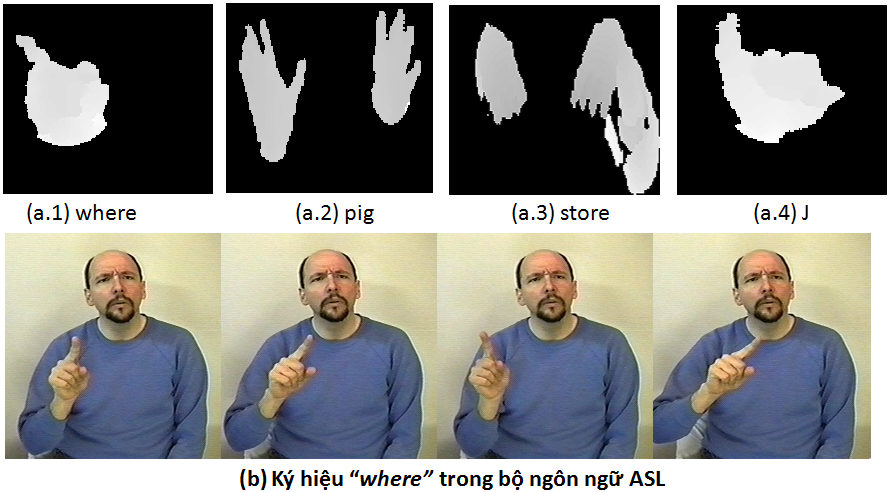
\includegraphics[scale=0.6]{gesture3d_samples.png}
\caption{a.1-4. Minh họa một số mẫu cử chỉ ASL trong tập dữ liệu MSRGesture3D, b. Chuỗi ảnh màu minh họa ký hiệu "\textit{where}" \cite{WangLCCW12_ROP}}
\label{fig_gesture3d}
\end{figure}

Đây là tập dữ liệu cử chỉ động của bàn tay thu được Kinect, và chỉ cung cấp duy nhất thông tin độ sâu. Tập dữ liệu này được thiết kế dựa trên tập ngôn ngữ ký hiệu ASL của Mĩ (\textit{American Sign Language}) \footnote{Cơ bản về ngôn ngữ ASL: http://www.lifeprint.com/asl101/pages-layout/concepts.htm}. Đặc điểm của tập dữ liệu như sau: 
\begin{itemize}
\item Gồm 12 lớp cử chỉ bàn tay và 10 chủ thể hành động khác nhau. Mỗi người thực hiện mỗi cử chỉ từ 2 đến 3 lần.
\item Có tổng cộng 336 mẫu dữ liệu độ sâu. % Độ phân giải mỗi mẫu là: 320 \(\times\) 240.
\item Tính chất: Các cử chỉ mang tính chất động, nghĩa là cả thông tin ngữ nghĩa về dáng \& chuyển động của bàn tay đều cần được dùng cho quá trình nhận dạng. Sự che khuất (Occlusion) xuất hiện rất nhiều trong tập dữ liệu.
\item Mỗi mẫu dữ liệu chỉ gồm chuyển động duy nhất của bàn tay (không bao gồm cổ tay). Hình \ref{fig_gesture3d} minh họa một số mẫu trong tập dữ liệu cùng diễn giải tương ứng về ý nghĩa của cử chỉ. 
\end{itemize}

\subsection{Cách thiết lập thí nghiệm}
Về tổng thể, cách thiết lập thí nghiệm trên tập MSRGesture3D gần giống với tập MSRAction3D - trình bày trong phần \ref{sec_action3d_exp}. Giải thuật \ref{alg_gesture_action3d} cũng trình bày chi tiết các bước thí nghiệm trên tập dữ liệu này.\\
Bên cạnh đó, một số thay đổi thiết lập như:
\begin{itemize}
\item Kích thước kim tự tháp không-thời gian được chọn là $4 \times 3 \times 3$ - bộ tham số này cho kết quả tốt hơn so với cách làm trên MSRAction3D, vì độ phân giải của tập dữ liệu này nhỏ hơn. 
\item Phương pháp đánh giá là kiểm chứng chéo sử dụng chiến lược "\textit{leave-one-out}", nghĩa là chỉ giữ lại duy nhất một chủ thể hành động để test và những người còn lại sẽ dùng cho việc huấn luyện. Cụ thể hơn, vì tập dữ liệu có 10 chủ thể hành động nên sẽ có tổng cộng tổ hợp $C_{10}^1 = 10$ thí nghiệm được thực hiện. Hiệu suất nhận dạng sẽ là độ chính xác trung bình xét trên tất cả các thí nghiệm. 
\end{itemize} 

\subsection{Kết quả thực nghiệm}
\begin{figure}
\centering
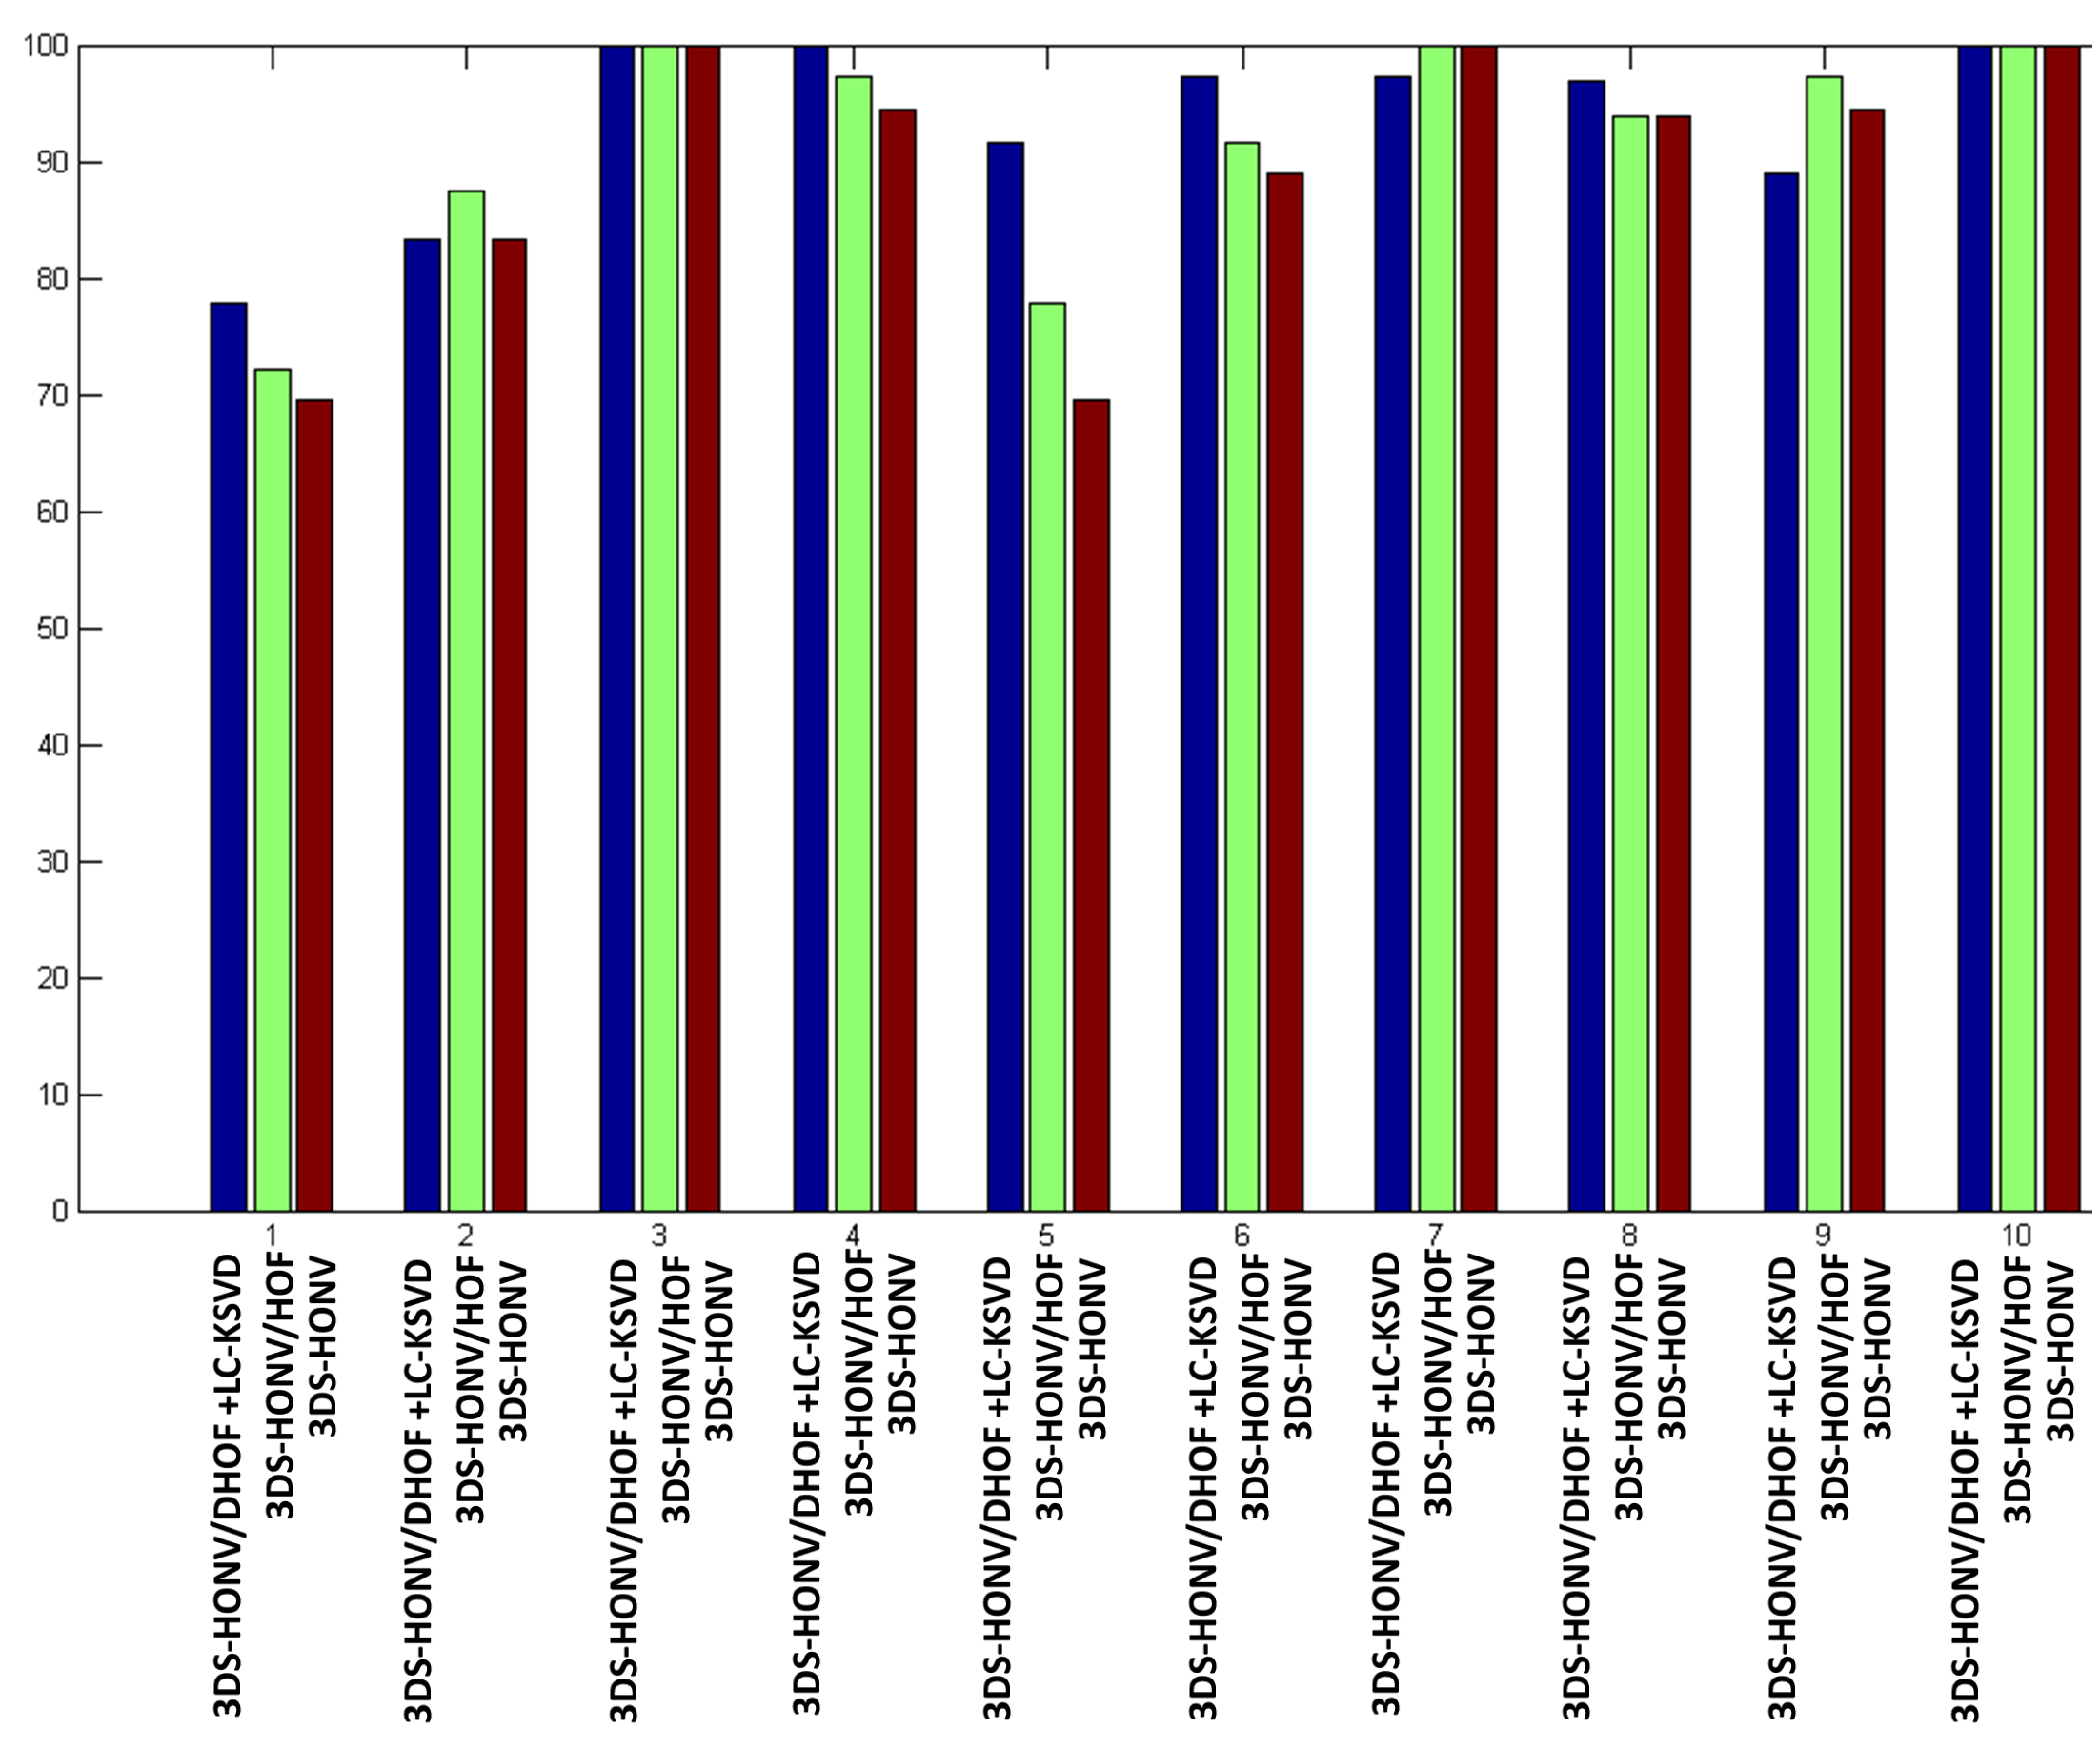
\includegraphics[scale=0.25]{gesture3d_graph.png}
\caption{Lược đồ so sánh độ chính xác phân lớp qua quá trình kiểm chứng chéo (10 thí nghiệm) của 3 loại đặc trưng đã đề xuất, xét trên tập dữ liệu MSRGesture3D}
\label{fig_gesture3d_graph}
\end{figure}

\begin{table}
	\caption{So sánh hiệu suất của các phương pháp đề xuất với các nghiên cứu khác trên tập dữ liệu MSRGesture3D}
	\centering 
	\begin{tabular}{l c}	
	\hline\hline
	\textbf{Phương pháp} & \textbf{Độ chính xác \%} \\	
	\hline\hline
	\textbf{3DSHONV-DHOF + sparse coding} & \textbf{93.31}\\ 
	\textbf{3DSHONV-DHOF (Our method)} &  \textbf{91.75}\\ 
	\textbf{3DS-HONV (Our method}) & \textbf{89.39}\\
	\hline \hline
	Omar et al. \cite{Omar_HON4D} (HON4D) & 87.29\\
	Omar et al. \cite{Omar_HON4D} (	HON4D + \(D_{disc}\))	&  92.45 \\
	Jiang et al. \cite{Wu_LOP2012} & 88.5 \\
	Yang et al. \cite{WangLCCW12_ROP} & 89.2 \\
	Klaser et al. \cite{Klaser_HOG3D} & 85.23 \\
	\hline
	\end{tabular}	
	\label{table_gesture3d}
\end{table}

Hình \ref{fig_gesture3d_graph} minh họa lược đồ thống kê và so sánh độ chính xác trung bình, xét trên tập dữ liệu MSRGesture3D, khi áp dụng 3 phương pháp trích chọn-biểu diễn đậc trưng là: 3DS-HONV, 3DSHONV-DHOF, và 3DSHONV-DHOF + SC (biểu diễn thưa của 3DSHONV-DHOF). Kết quả này được thống kê qua 10 thí nghiệm của quá trình kiểm chứng chéo "\textit{leave-one-out}". \\
Ta thấy rõ ràng đặc trưng kết hợp 3DSHONV-DHOF luôn cho độ chính xác cao hơn đặc trưng đơn 3DS-HONV xét trên tất cả các thí nghiệm. Trong khi đó, về tổng thể thì phương pháp biểu diễn thưa của đặc trưng 3DSHONV-DHOF đạt kết quả vượt trội so với các phương pháp còn lại trên đa số các thí nghiệm. Tuy nhiên, một số ngoại lệ xảy ra như ở thí nghiệm 2, 7 và 9, khi cách biểu diễn này lại cho kết quả tương đối thấp hơn 2 phương pháp còn lại. Điều này có thể lý giải là vì khóa luận đã sử dụng lại hoàn toàn các tham số codebook đã tối ưu trên tập dữ liệu MSRAction3D, cụ thể như kích thước từ điển là 200,... Dẫu vậy, nhìn chung độ chính xác trung bình của phương pháp biểu diễn thưa xét trên tập dữ liệu MSRGesture3D vẫn cao hơn 2 phương pháp còn lại và vượt trội so với bài báo state-of-art hiện tại \cite{Omar_HON4D} và một số nghiên cứu nổi bật khác. Kết quả này thống kê chi tiết trong bàng \ref{table_gesture3d}. 

Bên cạnh đó, một số điểm nổi bật có thể rút ra khi phân tích bảng số liệu \ref{table_gesture3d}. Xét trường hợp đặc trưng đơn 3DS-HONV, ta có thể thấy mặc dù với sự đơn giản và chi phí tính toán thấp, đặc trưng này cũng đem lại kết quả nhận dạng rất tốt (89.39\%) và cao hơn hầu hết các nghiên cứu trước đó. Cụ thể hơn, đặc trưng 3DS-HONV mà khóa luận trình bày chỉ đạt kết quả thấp hơn bài báo \cite{Omar_HON4D}, khi bài báo này áp dụng thêm một quy trình phức tạp và tốn kém để chuẩn hóa đặc trưng thông qua quá trình cập nhật \textit{score} của bộ phân lớp. Điều này thêm một lần nữa chứng minh tiềm năng mở rộng và áp dụng đặc trưng 3DS-HONV cùng các dạng thức kết hợp đặc trưng đã trình bày, cho các tác vụ nhận dạng cử chỉ-hành động tương tác thời gian thực trong tương lai.

%\section{Thí nghiệm trên tập dữ liệu MSRActivity3D}
%Tương tự tập dữ liệu MSRAction3D, tập MSRActivity3D cũng cung cấp 2 kênh thông tin là: độ sâu và khung xương. 

\section{Nhận dạng ngôn ngữ cử chỉ trên tập ChaLearn Gesture (CGD2011)\cite{chalearn_dataset}}
\label{chap_5_cgd}
\textit{Trong phần thí nghiệm này, khóa luận tiến hành phân tích, đánh giá lợi ích của việc kết hợp đặc trưng trích chọn từ nhiều kênh thông tin (màu-độ sâu) trên tập dữ liệu đa phương thức RGB-D, cụ thể là tập CGD2011. Qua thực nghiệm, khóa luận chứng minh rằng thông tin rút trích từ kênh dữ liệu màu và độ sâu là hoàn toàn bổ trợ nhau và đều cần thiết đề xây dựng phương thức biểu diễn cho một hệ thống nhận dạng bền vững, chính xác. Qua đó, khóa luận cũng cho thấy việc phát triển các nghiên cứu tiếp theo liên quan đến việc tìm kiếm các phương pháp khai thác, kết hợp hiệu quả nhiều kênh thông tin từ dữ liệu đa phương thức (RGB-D) là một hướng đi đúng đắn và tiềm năng.}
\subsection{Giới thiệu tập dữ liệu}
\subsubsection{Mô tả dữ liệu}
\begin{figure}
\centering
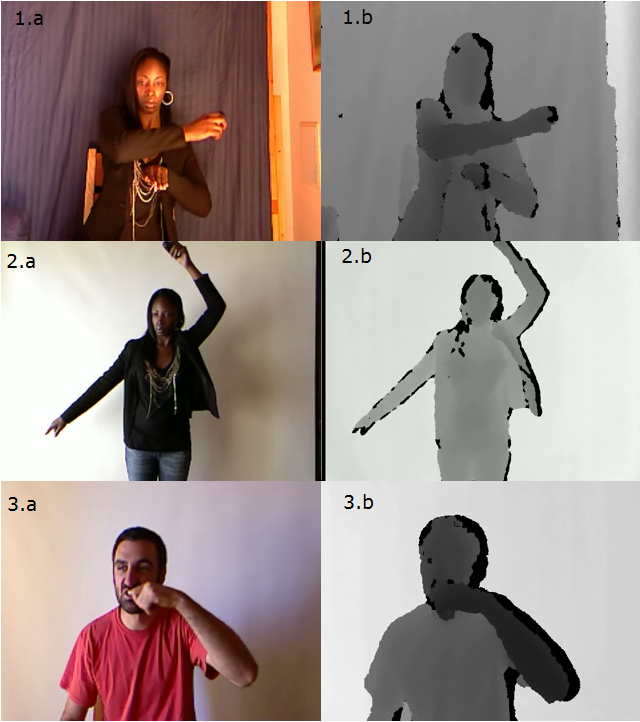
\includegraphics[scale=0.4]{cgd_samples.png}
\caption{Một số mẫu cử chỉ trích từ tập dữ liệu CGD2011: Hình 1 minh họa ngôn ngữ cử chỉ của người Ả-rập, hình 2 minh họa cử chỉ kêu gọi, hình 3 minh họa cử chỉ đánh răng. Các cặp hình a,b là các cặp ảnh màu-độ sâu tương ứng.}
\label{fig_cgd_samples}
\end{figure}
Đây là tập dữ liệu đa phương thức, bao gồm cả thông tin màu và độ sâu (RGB-D), được thu bằng Kinect (3D camera) và giới thiệu bởi Microsoft trong cuộc thi ChaLearn Gesture tổ chức vào năm 2011-2012 tại 2 hội nghị hàng đầu ICPR và CVPR \footnote{http://gesture.chalearn.org/}. \\
Tính chất của tập dữ liệu CGD2011 có thể được tóm tắt như sau: 
\begin{itemize}
\item Bao gồm tổng cộng 54,000 cử chỉ thực hiện chủ yếu bởi chuyển động của bàn tay và cánh tay người. Tập dữ liệu được tổ chức thành nhiều gói từ vựng con (gọi là batch), mỗi batch có kích thước từ vựng từ 8 đến 12 cử chỉ và được quay bởi một người dùng duy nhất. Số lượng mẫu tổng cộng trong mỗi batch gồm 47 mẫu video màu và 47 mẫu video độ sâu tương ứng. Một số ví dụ minh họa trong hình \ref{fig_cgd_samples}.
\item Định dạng của các mẫu dữ liệu:
	\begin{itemize}
		\item Kích thước frame: 240 \(\times\) 320 pixels
		\item Tần suất frame: 10 fps
	\end{itemize}
\item Trong mỗi batch, CGD2011 chỉ cung cấp duy nhất một mẫu huấn luyện cho mỗi lớp cử chỉ, vì vậy bài toán đặt ra trên dataset này thường được gọi là \textbf{One-shot-learning}, nghĩa là chỉ học một mẫu duy nhất cho mỗi lớp trong tác vụ nhận dạng.
\item Mỗi mẫu test tronng từng batch có thể bao gồm từ 1 đến 5 cử chỉ được thực hiện liên tục bởi cùng một người. Bên cạnh đó, tập dữ liệu cũng công bố thông tin chú giải (\textit{annotation}) và nhãn phân đoạn hành động theo thời gian (\textit{temporal segmentation}) trong 20 batch đầu (devel) của tập dữ liệu. \\
Dựa trên các nghiên cứu liên quan, khóa luận chỉ tập trung đánh giá hiệu suất mô hình đề xuất trên 20 batch đầu tiên (devel) của tập dữ liệu.
\end{itemize} 
Lược đồ minh họa cấu trúc tổ chức của tập dữ liệu cử chỉ CGD2011 được minh họa rõ nét trong hình \ref{fig_cgd_star}.


\begin{figure}
\centering
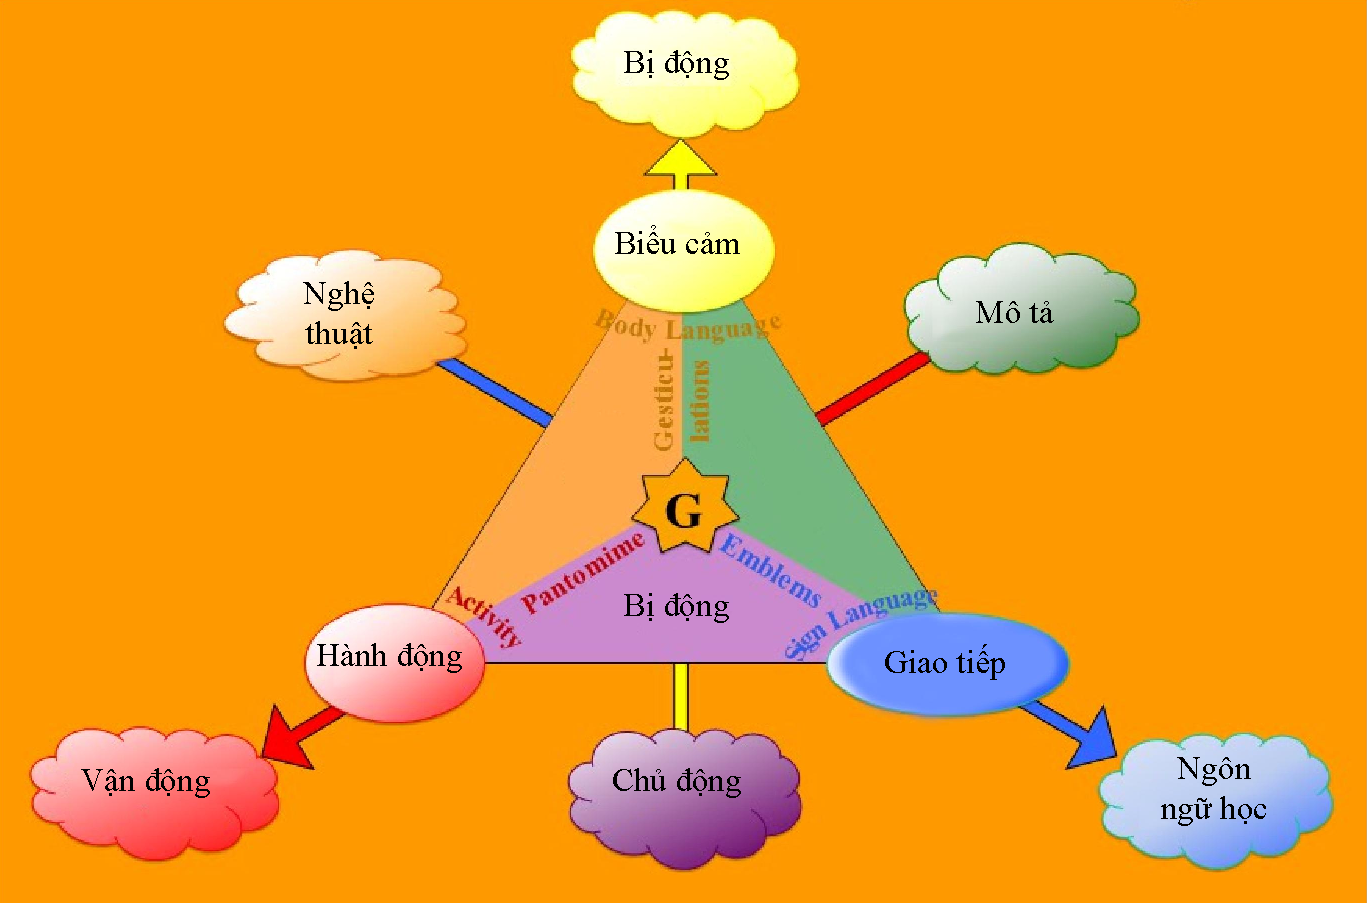
\includegraphics[scale=0.5]{cgd_star_gests.pdf}
\caption{Cấu trúc phân cấp các loại cử chỉ trong dataset CGD2011 \cite{chalearn_dataset}: Có thể chia thành 3 nhóm cử chỉ chính: Nhóm giao tiếp, biểu cảm và hành động. Các mẫu dữ liệu trong CGD được chọn lọc từ 85 tập từ vựng cử chỉ gồm: ngôn ngữ cử chỉ Ý, ngữ âm Ân Độ, ngôn ngữ cho người khiếm thính, cho thơ lặn, kịch câm, và ngôn ngữ cơ thể.}
\label{fig_cgd_star}
\end{figure}

\subsubsection{Độ đo đánh giá phương pháp}
Để đánh giá hiệu năng và so sánh độ chính xác giữa các phương pháp, CGD2011 đưa ra độ đo khoảng cách Levenshtein \cite{Leven_dist}, định nghĩa như sau: 
\begin{equation}
TeLev = \frac{{S + D + I}}{N}
\end{equation}
trong đó: 
\begin{itemize}
\item \(S\) (\textit{Substitutions}) là số lỗi phân lớp nhầm (\textit{misclassifications})
\item \(D\) (\textit{Deletions}) là số lỗi âm \textbf{false negative}
\item \(I\) (\textit{Insertions}) là số lỗi dương \textbf{false positive}
\item \(N\) là độ dài của chuỗi ground-truth.
\end{itemize}
Theo đó, độ đo Levenshtein trung bình càng thấp thì hệ thống nhận dạng càng tốt, và ngược lại. 

\subsubsection{Phân tich, nhận xét tập dữ liệu}
Về cơ bản, có 2 hướng tiếp cận có thể áp dụng để rút trích và biểu diễn thông tin cử chỉ trên tập CGD2011 là: Dựa trên phân tích thành phần cơ thể (\textit{Body parts}), hoặc sử dụng đặc trưng không gian-thời gian. Trước tiên, khóa luận phân tích ưu nhược điểm của các phương pháp trên: 
\begin{itemize}
\item \textbf{Hướng tiếp cận phân tích bộ phận: } Bước đầu tiên của hướng tiếp cận này là định vị các bộ phận của cơ thể (như đầu, vai, khuỷu tay, bàn tay). Một trong số nhưng phương pháp phổ biến nhất cho tác vụ này là sử dụng thuật toán "\textit{Rừng quyết định ngẫu nhiên}" (Randomized Decision Forests) được giới thiệu bởi nhóm nghiên cứu của Microsoft \cite{JamieShotton_Pose_recognition} và đã được tích hợp vào Kinect SDK để rút trích khung xương người. Tuy nhiên, trong tập dữ liệu CGD2011, thông tin về khung xương của chủ thể hành động lại không được cung cấp. Có thể nói việc phân tách được các cấu trúc bộ phận của cơ thể người từ các dữ liệu video đã thu sẵn với độ phân giải thấp là một bài toán vô cùng khó khăn và đầy thách thức. Một số phương pháp đã được đề xuất như \cite{EichnerMZF12_IJCV}, nhưng kết quả đạt được vẫn còn rất nhiều lỗi và chưa thỏa mãn cho các tác vụ tiếp theo.
\item \textbf{Hướng tiếp cận đặc trưng không gian-thời gian:} Với những phân tích về khuyết điểm của hướng tiếp cận theo bộ phận người, phương pháp được chọn trong khóa luận là dựa trên hướng tiếp cận đặc trưng không-thời gian. \\
Một số phương pháp tiêu biểu cho hướng tiếp cận này có thể kể đến như HOG\cite{Dalal_HOG}, HOF\cite{Dalal_HOF}. Tuy nhiên, theo khảo sát gần đây của \cite{Aggarwal_HAR_Review}, các nghiên cứu trước chủ yếu tập trung vào khai thác đặc trưng trên dữ liệu màu và vẫn còn tương đối ít các nghiên cứu trong việc trích chọn dạng biểu diễn thích hợp với dữ liệu độ sâu - đã và đang ngày càng phổ biến trong nhưng năm gần đây. Chính vì vậy đối với tập dữ liệu CGD2011, khóa luận tập trung vào việc thiết kế và kết hợp hiệu quả các đặc trưng thu được từ cả 2 kênh dữ liệu màu và độ sâu, từ đó dùng để học ra mô hình biểu diễn và phân lớp các cử chỉ-hành động. 
\end{itemize}

\subsection{Cách thiết lập thí nghiệm}
\begin{figure}
\centering
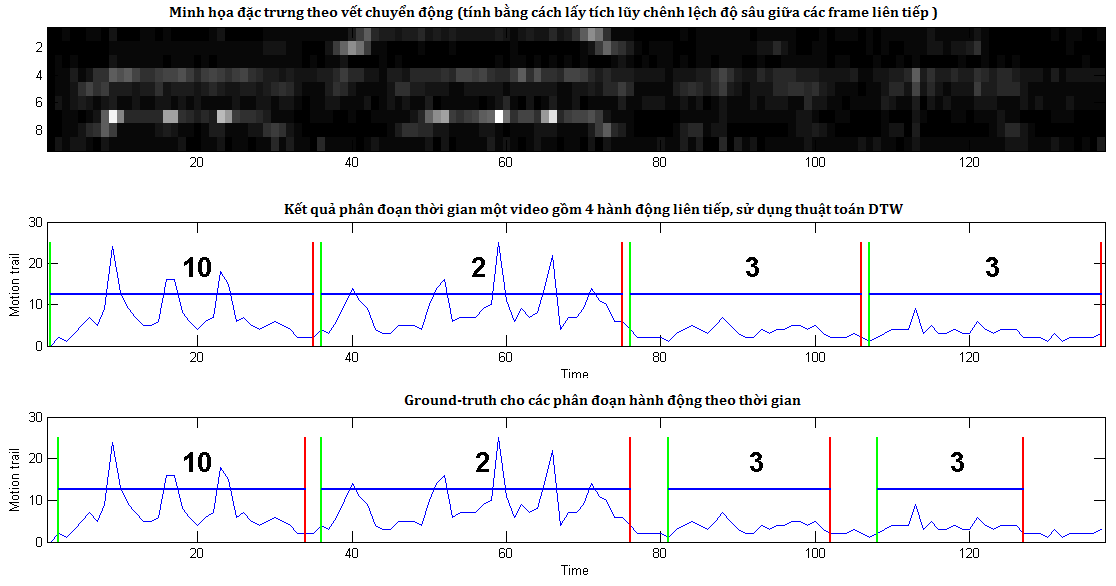
\includegraphics[scale=0.5]{dtw_res.png}
\caption{Hình minh họa khi sử dụng thuật toán DTW để phân đoạn thời gian một video gồm 4 hành động con liên tiếp. Đặc trưng được sử dụng để biểu diễn cho một phân đoạn hành động là vết chuyển động (tích lũy của \textit{frame difference})}
\label{fig_dtw_res}
\end{figure}
\begin{figure}
\centering
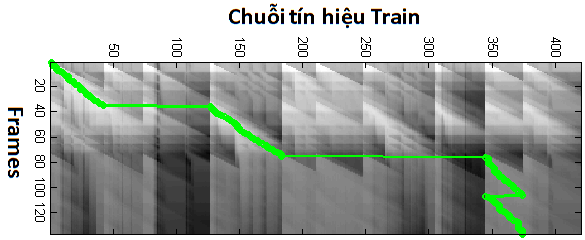
\includegraphics[scale=0.8]{dtw_seg.png}
\caption{Kết quả so khớp giữa tín hiệu kiểm thử (trục y) với các mẫu tín hiệu huấn luyện (trục x) sử dụng thuât toán DTW}
\label{fig_dtw_seg}
\end{figure}
Chi tiết quá trình thiết lập thí nghiệm trên tập dữ liệu CGD2011 được trình bày qua giải thuật \ref{alg_fusion_offline} cho giai đoạn huấn luyện (ngoại tuyến) và giải thuật \ref{alg_cgd2011} cho giai đoạn kiểm thử (trực tuyến). Về tổng thể, có thể thấy quy trình. Trong chương \ref{chap_4}, khóa luận đã giới thiệu chi tiết về mô hình trích chọn, kết hợp và biểu diễn đặc trưng trong giai đoạn ngoại tuyến; vì vậy trong phần này, khóa luận tập trung thảo luận rõ hơn các bước chính trong giai đoạn trực tuyến, xét trên tập dữ liệu cụ thể là CGD2011.

\subsubsection{Tiền xử lý dữ liệu kiểm thử}
Như đã trình bày, mỗi mẫu kiểm thử trong tập dữ liệu CGD2011 có thể bao gồm từ 1 đến 5 ngôn ngữ cử chỉ (tạm gọi chung là hành động) liên tiếp nhau. Chính vì vậy, trước khi vào giai đoạn nhận dạng, ta cần phải thực hiện thêm một công đoạn tiền xử lý, là phân chia chuỗi hành động liên tục này thành các hành động đơn lẻ. Một giải pháp phổ biến cho vấn đề này là sử dụng thuật toán \textbf{Dyanmic Time Warping (DTW)}\cite{Isabelle_Chalearn}. Về tổng quan, DTW là một phương pháp thuộc lớp thuật toán lập trình động (\textit{Dynamic Programming}), được sử dụng rất phổ biến trong cộng đồng xử lý tín hiệu số bởi tính hiệu quả của nó trong việc so khớp/ tìm kiếm các chuỗi tín hiệu tương tự nhau theo thời gian. Do phạm vi của khóa luận chủ yếu tập trung vào giới thiệu mô hình khai thác, biểu diễn đặc trưng có ngữ nghĩa trên dữ liệu màu và độ sâu, vì vậy giải thuật DTW sẽ không được trình bày chi tiết tại đây.

Hình \ref{fig_dtw_seg} mô tả quá trình so khớp chuỗi tín hiệu kiểm thử (trục \textit{y}) với các chuỗi tín hiệu trong tập huấn luyện (\textit{trục x}). Hình \ref{fig_dtw_res} minh họa kết quả phân đoạn thời gian 1 video gồm 4 hành động liên tiếp nhau. Trong minh họa này, đặc trưng vết chuyển động (tính bằng cách tích lũy sự chênh lêch độ sâu giữa các khung hình liên tiếp) được sử dụng để miêu tả cho một chuỗi hành động (tín hiệu) đơn và dùng làm tập mẫu so khớp cho giải thuật DTW. Chi tiết về thuật toán này được trình bày trong bài báo \cite{Isabelle_Baseline}. Nhìn chung kết quả phân đoạn chuỗi hành động liên tiếp theo thời gian dựa trên thuật toán DTW là khá chính xác và đủ thỏa mãn để thực hiện các tác vụ nhận dạng tiếp theo.  

\subsubsection{Các tham số cài đặt giải thuật \ref{alg_cgd2011}}
\begin{itemize}
	\item Bước trích đặc trưng: Kích thước của cửa sổ cục bộ (\textit{space-time volume}) xung quanh các điểm trọng yếu STIPs được tính như sau: $\delta_x=\delta_y=2k\sigma,\hspace{0.05in}\delta_t=2k\tau$, trong đó $\sigma, \tau$ lần lượt là mức scale theo không-thời gian của cửa sổ (xem chương \ref{chap_3}). Mỗi cửa sổ xung quanh các STIP sẽ được chia thành 1 lưới $n_x \times n_y\times n_t$ cửa sổ con. Theo đó, các đặc trưng như HOG, HOF, HOF2.5D và 3DS-HONV sẽ lần lượt được rút trích tại các cửa sổ cục bộ này với tham số thiết lập như sau: 
		\begin{itemize} 
			\item Tham số $k=9$ được cài đặt cố định cho mọi trường hợp. (theo gợi ý Laptev\cite{LMSR08})
			\item Đối với đặc trưng HOG, HOF: , $n_x = n_y = 3$, $n_t = 2$. Kích thước bins của HOG là 4 và HOF là 5. Như vậy, kích thước sau cùng của đặc trưng HOG mô tả cho 1 điểm trọng yếu STIP là: $3\times 3\times2\times4 = 72$, tương tự cho HOF là 90 (bins). 
			\item Đối với đặc trưng HOF2.5D: $n_x = n_y = 2$, $n_t=1$. Kích thước bins của HOF2.5D cho mỗi mặt lần lượt là 8. Như vậy, số chiều của HOF2.5D tại mỗi STIP là: $(2\times2\times1)\hspace{0.05in}\times\hspace{0.05in}(8+8+8)=96$ (bins) (xem chi tiết trong chương \ref{sec_dhof})
			\item Đối với đặc trưng 3DS-HONV: $n_x = n_y = n_t = 1$. Kích thước bins của 3DS-HONV trên không gian tọa độ cầu lần lượt là: $b_\theta=5,b_\phi=5,b_\psi=6$. Như vậy số chiều của đặc trưng 3DS-HONV tại mỗi STIP là 150. (chi tiết trong chương \ref{sec_shonv})
		\end{itemize}
	\item Kích thước kim tự tháp không-thời gian chia trên video là $2\times2\times2$ khối thể tích con (cells). Ở đây, khóa luận sử dụng lại bộ tham số tốt nhất mà Laptev đã thử nghiệm cho hướng tiếp cận đặc trưng cục bộ không-thời gian STIP\cite{LMSR08}). 
	\item Kich thước từ điển cho quá trình tạo codebook tại từng khối thể tích con (cells) sử dụng thuật toán SC là 200 (từ), cho cả các loại đặc trưng màu-độ sâu, cụ thể như: HOG, HOF, HOG-HOF, HOF2.5D, HOG-HOF2.5D và 3DS-HONV. 
	\item Giá trị vô hướng $\alpha=0.8$, dùng để đánh trọng số mức độ ảnh hướng của các loại đặc trưng lên kết quả phân lớp.
\end{itemize}

	\begin{algorithm}
	\newalgname{Giải thuật}
	\caption{Giải thuật giai đoạn trực tuyến (rút trích-biểu diễn đặc trưng \& phân lớp) cho bài toán "\textit{One-shot-learning}" trên tập dữ liệu đa phương thức \textbf{CGD2011}\cite{chalearn_dataset}}
	\label{alg_cgd2011}
	Ràng buộc bài toán "\textit{One-shot-learning}" trên tập CGD2011: Có đúng $M$ mẫu huấn luyện (gồm thông tin màu và độ sâu) cho $M$ lớp cử chỉ (\textit{mỗi lớp một mẫu huấn luyện}).
	{\fontsize{12}{12}\selectfont
	\begin{algorithmic}
	\renewcommand{\algorithmicrequire}{\textbf{Đầu vào:}}
	\renewcommand{\algorithmicensure}{\textbf{Đầu ra:}}
	\algnewcommand\algorithmicoperation{\textbf{Thao tác:}}
	\algnewcommand\Operation{\item[\algorithmicoperation]}
	
	\Require 
	\State M mẫu huấn luyện (RGB-D video): \(T_r = \{t_{r1},...,T_{rM}\}\)	
	\State Tập vector đặc trưng rút từ các mẫu huấn luyện: \(H_{r}^F = \{h_{r1}^F,...h_{rM}^F\}\) (tính từ tầng huấn luyện)
	\State Tập Codebook đã học: \(B\) (được tính từ bước huấn luyện).
	\State 1 mẫu test (RGB-D video): \(t_e = \{t_{e_{i=1..N}}\} \in \mathbb{R}^N\), với $N=[1..5]$
	
	\Ensure 
	\State Kết quả nhận dạng: \textit{Lóp cử chỉ ($class$)}
	
	\Operation \\	
	\begin{enumerate}		
		\item Tiền xử lý: (a) Loại nhiễu trên ảnh độ sâu sử dụng bộ lọc song phương (\textit{bilateral filter} \cite{camplani_jbf}). Cân chỉnh 2 dữ liệu màu-độ sâu (calibration/ image alignment).
		\item Khởi tạo: $class = [\hspace{0.05in}]$
		\item Phân đoạn cử chỉ theo thời gian: $\{t_{e_1},t_{e_2},...,t_{e_N}\} = DTW(T_r,t_e)$
		\For{$i=1;i\le N;i++$}		
			\State Chia $t_{e_i}$ thành $n_c = n_x\times n_y\times n_t$ khối con (cells) tuần tự theo hệ trục $x,y,t$			
			\State Dò tìm điểm trọng yếu Harris3D\cite{Laptev_STIP}: $\{STIPs\}_{t_{e_i}}^F$ với $F \in \{RGB, D\}$ (RGB: kênh màu, D: kênh độ sâu) 			
			\State Tại mỗi $STIP^F$, tính đặc trưng \textbf{3DS-HONV} với $F=RGB$, tính \textbf{HOG} với $F=D$ và tính \textbf{HOF2.5D} với $F={RGB,D}$. Kết hợp đặc trưng HOG và HOF2.5D thành HOG-HOF2.5D tại $STIP^{RGB}$.
			\State Tính lược đồ phân bố $STIPs^F$ tại mỗi cell: 
			\begin{equation}
				\begin{array}{l}			
				h^{RGB}_{c_{j=1..n_c}} = \sum\limits_{p\in c_j} h_p^{HOG-HOF2.5D} \hspace{0.1in}s.t.\hspace{0.1in} p \in \{STIPs\}^{RGB}\\
				h^{D}_{c_{j=1..n_c}} = \sum\limits_{q\in c_j} h_q^{3DS-HONV} \hspace{0.1in}s.t.\hspace{0.1in} q \in \{STIPs\}^{D}				
				\end{array}				
			\end{equation}
			\State Tính biểu diễn thưa $X^{F=\{RGB,D\}}$ của $h^{F=\{RGB,D\}}$ dựa trên codebook $B$, sử dụng thuật toán SC
%			\begin{equation}
%				\begin{array}{l}
%				 < D,A,X >  = \arg \mathop {\min }\limits_{D,A,X} \left\| {{h^{te}_j} - DX} \right\|_2^2\\
%				 \hspace{0.8in} + \alpha \left\| {Q - AX} \right\|_2^2 \hspace{0.15in} s.t.\forall k,{\left\| {{x_k}} \right\|_0} \le T
%				\end{array}
%			\end{equation}
			\State Tính hist $h_i^{F} = \mathop  \odot \limits_{j = 1..{n_c}} h_{c_j}^{F} \hspace{0.1in}s.t.\hspace{0.1in} F=\{RGB,D\}$ để biểu diễn cho $t_{e_i}$ (\gls{acr_concate} là toán tử nối vector)
			\State \textbf{Pha Phân lớp}: kNN-classifier, độ đo \textit{histogram intersection}
			%$d_i^F = kNN\_classify(H_i^F, H_r^F) \hspace{0.1in}s.t.\hspace{0.1in} F=\{RGB,D\}$ 		
%			\resizebox{.4\hsize}{!}{$ d_i^F = 1 - \frac{{\sum\limits_k {\min \left((h_i^F(k),H_r^F(k)\right)} }}{{\min \left( {\sum\limits_k {h_i^F(k)}, \sum\limits_k {H_r^F(k)} } \right)}} $}
			\begin{equation}
				\begin{array}{l}
			d_i^F = 1 - {{\sum\limits_k {\min \left( {(h_i^F(k),H_r^F(k)} \right)} } \mathord{\left/
			 {\vphantom {{\sum\limits_k {\min \left( {(h_i^F(k),H_r^F(k)} \right)} } {\min \left( {\sum\limits_k {h_i^F(k)} ,\sum\limits_k {H_r^F(k)} } \right)}}} \right.
			 \kern-\nulldelimiterspace} {\min \left( {\sum\limits_k {h_i^F(k)} ,\sum\limits_k {H_r^F(k)} } \right)}}\\ \\
			\textbf{Late - fusion:}\hspace{0.1in}d_i = \alpha \cdot d_i^{\textbf{D}} + (1-\alpha)\cdot d_i^{\textbf{RGB}} \hspace{0.1in}\textbf{=>\hspace{0.1in} tmp\_class}
				\end{array}
			\end{equation}
			\State $class = [class\hspace{0.1in} tmp\_class]$
		\EndFor \\
		\Return \textit{class}	
	\end{enumerate}		
	\end{algorithmic}
	}
	\end{algorithm}

\subsection{Kết quả thực nghiệm}	
\begin{figure}
\centering
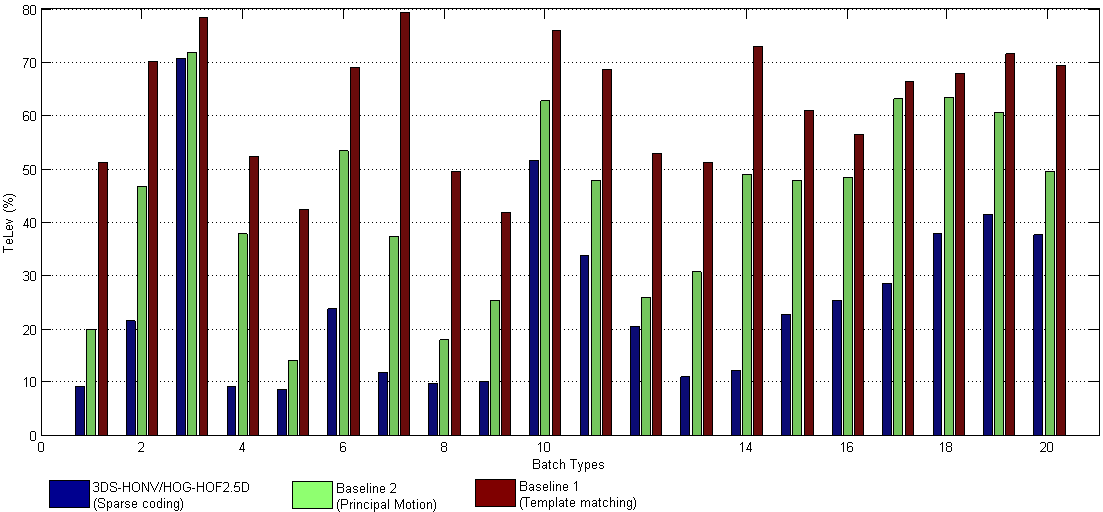
\includegraphics[scale=0.5]{CGD_results.png}
\caption{So sánh hiệu suất mô hình kết hợp đặc trưng được trình bày trong giải thuật \ref{alg_cgd2011} với các phương pháp cơ sở (baseline)\cite{Isabelle_Chalearn}, \cite{Isabelle_Baseline}, xét trên 20 bộ (batch) đầu của tập dữ liệu CGD2011\cite{chalearn_dataset}. Trục X thể hiện các batch khác nhau, Y mô tả độ đo Levenshtein trung bình trên từng batch.}
\label{fig_cgd_results}
\end{figure}
Bảng \ref{table_CGD_result} thống kê hiệu suất khi sử dụng đơn lẻ từng loại đặc trưng màu, độ sâu và khi kết hợp cả 2 nguồn thông tin này cho bài toán nhận dạng cử chỉ trên tập CGD2011; quy trình thực nghiệm tuân theo 2 giải thuật \ref{alg_fusion_offline} và \ref{alg_cgd2011}. Cần nhấn mạnh rằng, các đặc trưng được trích chọn và kết hợp trong bảng \ref{table_CGD_result} đều đã qua quá trình biểu diễn thưa sử dụng codebook học bởi thuật toán SC. Phân tích bảng số liệu, ta có thể rút ra nhận xét sau: 
\begin{itemize}
\item Đặc trưng HOF rút trên kênh dữ liệu màu cho kết quả nhận dạng thấp nhất (TeLev = 41.44\%). Trong khi đó, đặc trưng HOG cho kết quả cao hơn (34.52\%) và phiên bản kết hợp (\textit{early fusion}) của HOG và HOF (HOG-HOF) cho kết quả tốt nhất (33.14\%), xét trong trường hợp chỉ sử dụng thông tin từ kênh dữ liệu RGB. Kết quả thu được cho thấy việc khai thác phân bố về dáng trong không-thời gian (HOG) sẽ giúp mô tả tốt hơn các cử chỉ trong tập dữ liệu (xem hình \ref{fig_gest_demo}(1-3))so với khi chỉ sử dụng thông tin chuyển động (HOF). Bên cạnh đó, ta cũng có thể thấy việc kết hợp cả dáng và chuyển động để biểu diễn cho 1 hành động/ cử chỉ là rất quan trọng và giúp cải thiện đáng kể hiệu suất nhận dạng. 
\item Xét trên kênh dữ liệu độ sâu, đặc trưng 3DS-HONV mà khóa luận đề xuất cho kết quả vượt trội (TeLev = 28.91\%) so với các đặc trưng rút trích trên kênh RGB. Điều này có thể lý giải vì đặc trưng 3DS-HONV có thể trích chọn hiệu quả các thông tin liên hợp về dáng-chuyển động trong không gian 4 chiều ($x-y-z-t$). Tính chất này giúp cho đặc trưng 3DS-HONV không chỉ biểu diễn tốt các cử chỉ phụ thuộc nhiều vào sự thể hiện về dáng, mà còn có thể phân tách tốt các cử chỉ có nhiều chuyển động trong không gian ($x-y-z$) qua thời gian (ví dụ, cử chỉ có chuyển động của tay từ sau ra trước và ngược lại, xem hình \ref{fig_gest_demo} (4.a-4.c)).
\item Với các phân tích nêu trên, ta có thể dễ dàng suy luận việc kết hợp các đặc trưng từ 2 kênh dữ liệu màu-độ sâu có thể đem lại các kết quả tích cực. Điều này đã được chứng mình qua thực nghiệm, theo bảng, ta thấy đặc trưng HOF2.5D - tính nhờ sử dụng kết hợp cả thông tin RGB và độ sâu, cho kết quả vượt trội so với đặc trưng HOF truyền thống (trên kênh RGB). Một cách tự nhiên, khi ta tăng cường thêm khả năng biểu diễn dáng của HOG vào HOF2.5D, đặc trưng kết hợp thu được HOG-HOF2.5D (\textit{early fusion}) cho kết quả tốt hơn (30.27\%) so với HOG-HOF thông thường. 
\item Cuối cùng, ta có thể thấy chiến lược kết hợp trễ (\textit{late fusion}) các biểu diễn thưa của đặc trưng 3DS-HONV và HOG-HOF2.5D (mô hình đề xuất chính của khóa luận) cho kết quả hoàn toàn vượt trội (24.89\%) so với các đặc trưng đơn lẻ, hay các dạng kết hợp đặc trưng kết hợp sớm (\textit{early fusion}). Điều này có thể lý giải là vì chiến lược kết hợp trễ đã tận dụng được tốt sức mạnh phân lớp từ cả 2 loại đặc trưng 3DS-HONV và HOG-HOF2.5D. Cụ thể hơn, đặc trưng 3DS-HONV có khả năng biểu diễn rất tốt các thông tin về dáng và chuyển động (nhất là các chuyển động theo truc $z$) của đối tượng trong không gian 3 chiều $x,y,z$; trong khi đó, đặc trưng HOG-HOF2.5D có thể đặc tả được thông tin liên tục về dáng cũng như lưu giữ tốt các thông tin chuyển động trong mặt phẳng ảnh (\textit{in-plane motions}). Có thể nói 2 đặc trưng này có thể tương hỗ cho nhau, và việc sử dụng chiến lược kệt hợp trễ - với tham số đánh giá mức độ ảnh hưởng ($\alpha$) phù hợp, là hoàn toàn hợp lý để tận dụng tối đa sức mạnh phân lớp của từng loại đặc trưng. 
\end{itemize}

\begin{figure}
\centering
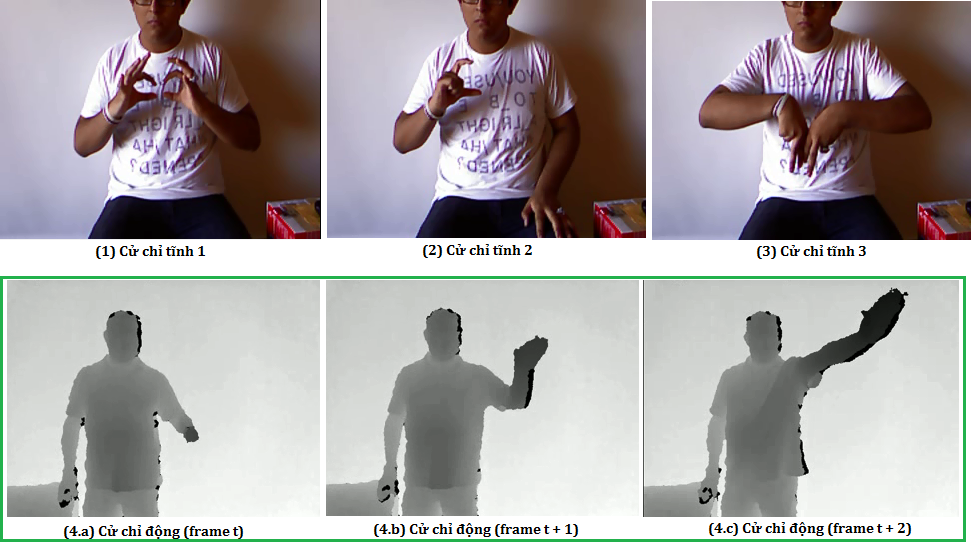
\includegraphics[scale=0.5]{gest_demo.png}
\caption{Minh họa 1 số cử chỉ trích từ tập CGD2011: (Hình 1-3) là ảnh RGB minh họa 3 loại cử chỉ tĩnh khác nhau-phụ thuộc nhiều thông tin về dáng; (Hình 4.(a-c) là ảnh độ sâu minh họa 1 chuỗi cử chỉ động theo thời gian - mang nhiều thông tin chuyển động theo không gian $x-y-z$.)}
\label{fig_gest_demo}
\end{figure}
Qua kết quả đạt được, khóa luận cũng tiến hành so sánh hiệu suất tốt nhất của mô hình đề xuất so với các nghiên cứu nổi bật khác xét trên tập dữ liệu CGD2011. Bảng \ref{table_CGD_result} cho thấy phương pháp của khóa luận đã đạt được kết quả rất đáng khich lệ, khi thực nghiệm trên 20 bộ cử chỉ đầu (\textit{devel}) của tập CGD và đạt độ lỗi Levenshtein trung bình thấp hơn nhiều so với 2 phương pháp chuẩn (baseline) của tập dữ liệu, cũng như một số phương pháp nổi bật khác được công bố gần đây. Hình \ref{fig_cgd_results} là đồ thị thống kê và so sánh độ lỗi Levenshtein trung bình của phương pháp trình bày so với 2 phương pháp baseline \cite{Isabelle_Chalearn}, \cite{Isabelle_Baseline} đề xuất bởi các tác giả thiết kế tập dữ liệu CGD2011. 

\begin{table}
	\caption{Đánh giá hiệu suất khi sử dụng riêng lẻ và kết hợp từng loại đặc trưng trên các kênh dữ liệu màu-độ sâu)}
	\centering 
	\scalebox{1}{
	\begin{tabular}{|l | c || c | c || c | c |}	
	\hline
	\textbf{RGB Desc.} & \textbf{TeLev\%} & \textbf{Depth Desc.} & \textbf{TeLev} & \textbf{RGB-D Desc.} & \textbf{TeLev}\\	
	\hline\hline
	HOG & 34.52 & 3DS-HONV & 28.91 & HOF2.5D & 33.52 \\
		HOF & 41.44 & & & HOG-HOF2.5D & 30.27 \\
	HOG-HOF	& 33.14 & & & 3DS-HONV/HOG-HOF2.5D & 24.89 \\
	\hline
	\end{tabular}	}
	\label{table_CGD_result}
\end{table}

\begin{table}
	\caption{So sánh độ chính xác với một số nghiên cứu nổi bật khác, xét trên 20 batch "devel" của tập CGD2011, sử dụng độ đo Levenshtein.}
	\centering 
	\scalebox{1}{
	\begin{tabular}{|l | c |}	
	\hline
	\textbf{Phương pháp} & \textbf{TeLev \%} \\	
	\hline\hline
	\textbf{3DS-HONV/HOG-HOF2.5D (Sparse coding)} (\textbf{đề xuất})& \textbf{24.89 }\\
	\hline\hline
	Baseline 1 (Template matching) \cite{Isabelle_Chalearn} & 62.31 \\
	Baseline 2 (PCA-based: Principal motion) \cite{Isabelle_Baseline} & 43.63 \\
	Manifold LSR \cite{YuiManLui_least_squares_gesture} & 28.73 \\
	MHI \cite{WuZS12_cvpr} & 30.01 \\
	Extened-MHI \cite{WuZS12_cvpr} & 26.00 \\
	\hline
	\end{tabular}	}
	\label{table_CGD_comparison}
\end{table}

\section{Chương trình ứng dụng minh họa}
Trong phần này, khóa luận giới thiệu sơ lược về 1 số ứng dụng thực tiễn đã phát triển dựa trên mô hình trích chọn-kết hợp đặc trưng đã giới thiệu cho bài toán nhận dạng hành động người. 

\subsection{Ứng dụng nhận dạng hành động-ngôn ngữ cử chỉ người theo thời gian thực}
\begin{figure}
\centering
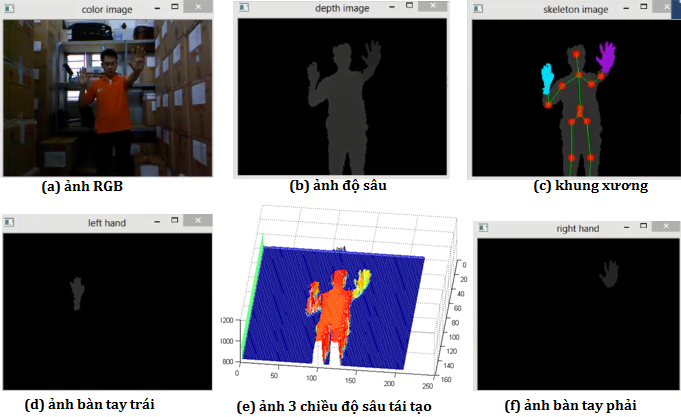
\includegraphics[scale=0.8]{real_demo_gesture.png}
\caption{Minh họa ứng dụng nhận dạng hành động thời gian thực sử dụng Kinect}
\label{fig_real_gest_demo}
\end{figure}
\subsubsection{A. Giới thiệu ứng dụng:}
\begin{itemize}
	\item \textbf{Môi trường phát triển:} Windows 7-8, C++
	\item \textbf{Thiết bị phụ trợ:} Kinect
	\item \textbf{Các thư viên sử dụng:} OpenCV, KinectSDK, YARP (thư viên xử lý tính toán ma trận, dùng nhiều trong lĩnh vực robotics)
	\item \textbf{Tập dữ liệu :} Do khóa luận tự thiết kế
	\item \textbf{Chức năng:} Nhận dạng chuỗi hành động liên tục trong thời gian thực
	\item \textbf{Sơ lược về phương pháp: } 
		\begin{itemize}
			\item Các module chính: (1) Rút trích khung xương của người và dò tìm bàn tay của người trong khung cảnh; (2) Trích chọn đặc trưng, (3) Huấn luyến \& phân lớp hành động bằng thuật toán SVM
			\item Các đặc trưng được sử dụng: (1) Đặc trưng HOG được rút trích xung quanh các vùng bàn tay, đặc trưng 3DS-HONV toàn cục mô tả thông tin về dáng của người; (2) đặc trưng HOF2.5D (\textit{semi-scene flow}) được rút trên toàn vùng ảnh quan sát theo thời gian.
			\item Bộ phân lớp sử dụng: SVM tuyến tính (\textit{Linear SVM}).
		\end{itemize}		
\end{itemize}

\subsubsection{B. Giới thiệu tập dữ liệu thử nghiệm \& Quy trình nhận dạng}
\begin{figure}
\centering
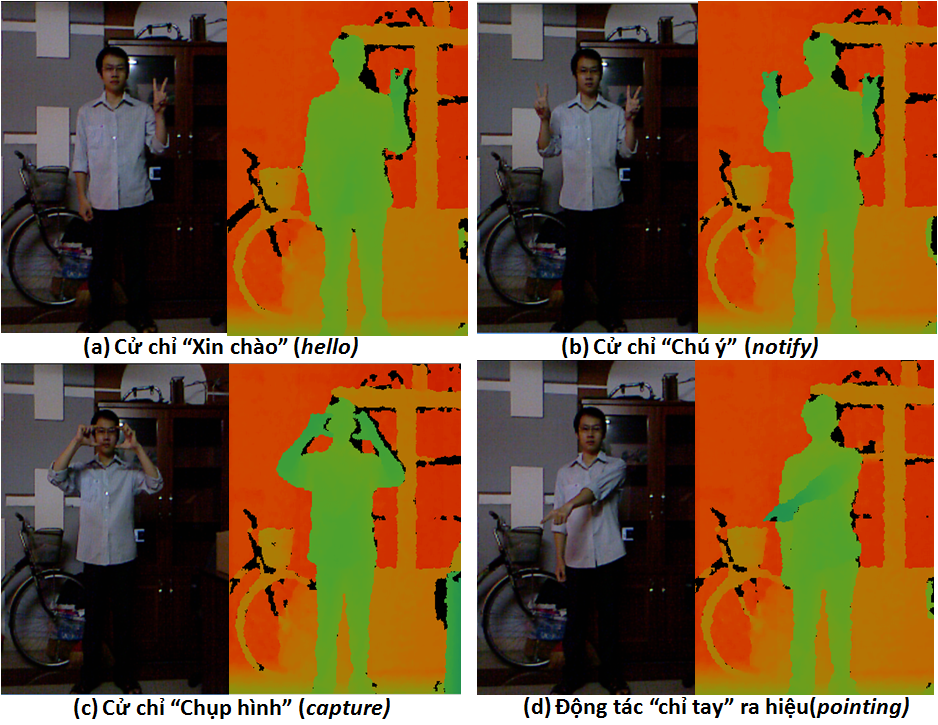
\includegraphics[scale=0.65]{real_demo_train.png}
\caption{Minh họa tập 4 mẫu hành động huấn luyện do khóa luận tự tạo}
\label{fig_real_demo_train}
\end{figure}
\begin{enumerate}
	\item \textbf{Tập dữ liệu thử nghiệm: }
		\begin{itemize}
			\item Do khóa luận tự đinh nghĩa và quay. 
			\item Gồm có 4 lớp hành động chính trong tập dữ liệu, mỗi hành động chỉ có một mẫu huấn luyện duy nhất(Xem hình \ref{fig_real_demo_train}).
			\item Lưu ý: Các mẫu huấn luyện có tính chất: 2 tay của người thực hiện hành động phải duỗi thẳng tại frame bắt đầu và frame kết thúc của mỗi mẫu (xem hình \ref{fig_real_demo_signal}).
		\end{itemize}
	
%	\item \textbf{Quy trình nhận dạng theo thời gian thực}	
\begin{figure}
\centering
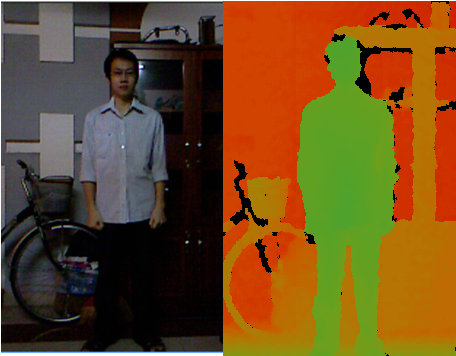
\includegraphics[scale=0.7]{real_demo_signal.png}
\caption{Minh họa tư thế bắt đầu và kết thúc cho mỗi chuỗi hành động-cử chỉ đơn.}
\label{fig_real_demo_signal}
\end{figure}	
		\item \textbf{Quy ước:} Các hành động có thể được thực hiện liên tục theo thời gian. Trạng thái bắt đầu và kết thúc của mỗi hành động cũng phải tuân theo quy ước của các mẫu huấn luyện là: 2 tay của người thực hiện hành động phải ở tư thế duỗi thẳng.
		\item Về tổng quan, để phân đoạn chuỗi hành động thành các hành động đơn lẻ, khóa luận sử dụng kỹ thuật quét cửa sổ theo thời gian (kích thước khoảng 30 frame một cửa sổ) để rút trích đặc trưng và nhận dạng liên tục các hành động trong chuỗi cửa sổ đó.
		\item Hình \ref{fig_real_gest_demo} minh họa các kết quả dò tìm các vùng bàn tay của người, rút trích khung xương và hình ảnh 3D tái tạo hành động của người trong thế giới thực. Sau quá trình dò tìm các vùng bàn tay, đặc trưng HOG sẽ được rút trích xung quanh các vùng bàn tay trên ảnh độ sâu, trong khi đó đặc trưng 3DS-HONV và HOF2.5D sẽ được trích chọn trên toàn vùng ảnh để mô tả cho hành động đó. Do tính chất đơn giản của các đặc trưng (đã chứng minh ở chương \ref{chap_3}), việc rút trích đặc trưng \& phân lớp các hành động có thể tiến hành trong thời gian thực, đồng thời vẫn đảm bảo độ chính xác cao.\\
		Do số lớp hành động mà khóa luận sử dụng cho mục đích huấn luyện và thí nghiệm là ít, vì vậy độ chính xác của phương pháp nhận dạng hiện tại là tương đối cao.
\end{enumerate}

\subsection{Ứng dụng game tương tác luyện trí nhớ qua ngôn ngữ bàn tay}
\begin{figure}
\centering
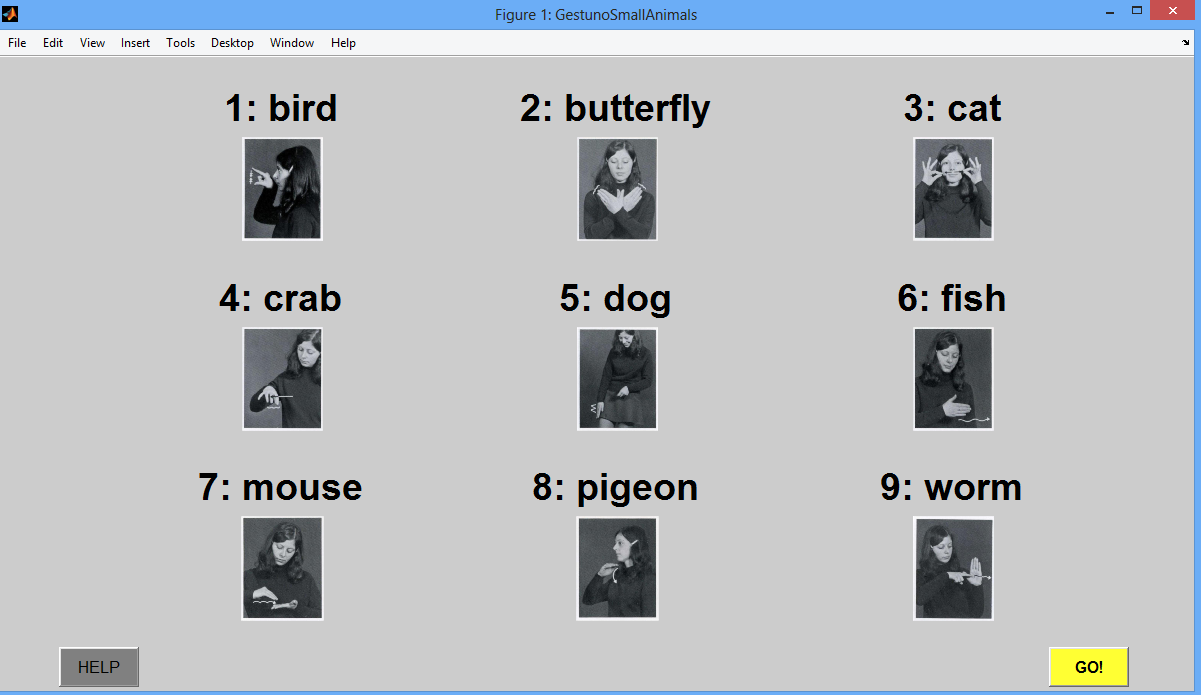
\includegraphics[scale=0.5]{cgd_lexicon.png}
\caption{Minh họa 1 tập dữ liệu gồm các ngôn ngữ cử chỉ sẽ được dùng để dạy cho người chơi trong game luyện trí nhớ}
\label{fig_cgd_lexicon}
\end{figure}

\subsubsection{Giới thiệu ứng dụng:}
\begin{figure}
\centering
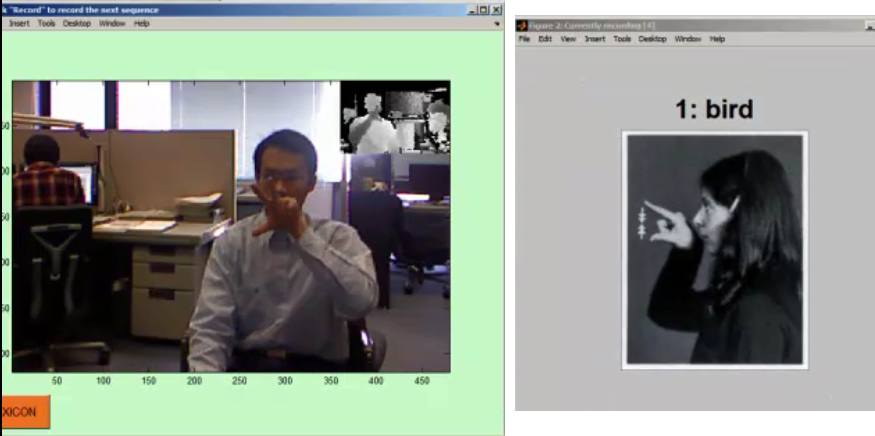
\includegraphics[scale=0.7]{game_demo_1.png}
\caption{Minh họa game tương tác luyện trí nhớ sử dụng ngôn ngữ cử chỉ: Đối tượng đang thực hiện ngôn ngữ cử chỉ mô tả con chim (bird) - đã được huấn luyện trước đó.}
\label{fig_game_gest_1}
\end{figure}

\begin{itemize}
	\item \textbf{Môi trường phát triển: } Windows 7-8, Matlab
	\item \textbf{Thiết bị phụ trợ:} Webcam thông thường hoặc Kinect
	\item \textbf{Thư viện sử dụng: } Bộ thư viên các hàm xử lý ảnh do \textbf{Isabelle Guyon} thiết kế để hỗ trợ cho việc truy cập và khai thác thông tin trên tập dữ liệu CGD2011 \cite{Isabelle_Chalearn}.
	\item \textbf{Chức năng của chương trình: } Hỗ trợ người chơi trong việc học các ngôn ngữ ký hiệu qua một trò chơi tương tác qua lại giữa người và máy. 
		\begin{itemize}
			\item Đầu tiên, chương trình hiển thị một danh sách hình minh họa các ngôn ngữ cử chỉ cùng ý nghĩa tương ứng. Người chơi sẽ phải quan sát và ghi nhớ danh sách tên cùng hành động mô tả của các cử chỉ này. (xem hình \ref{fig_cgd_lexicon})
			\item Sau đó, chương trình sẽ lần lượt duyệt qua các mô tả cử chỉ trong tập dữ liệu, hiển thị để người chơi quan sát và thực hiện hành động mô tả cử chỉ trong ảnh (xem hình \ref{fig_game_gest_1}). Quá trình này được thiết kế nhằm mục đích: vừa để người chơi ghi nhớ từng ngôn ngữ cử chỉ, vừa để tạo dữ liệu mẫu (train) cho bộ huấn luyện phân lớp cử chỉ của chương trình.
			\item Sau quá trình huấn luyện người chơi trên, chương trình sẽ lần lượt hiển thị tên các cử chỉ trong tập dữ liệu và yêu cầu người chơi phải thực hiện lại đúng hành động mô tả cử chỉ đó. Nếu người chơi thực hiện đúng, kết quả thu được sẽ như hình \ref{fig_game_gest_2}. Về bản chất, mục đích của quá trình này được dùng để kiểm định hiệu năng của bộ phân lớp đã huấn luyện.
		\end{itemize}
	\item Sơ lược về phương pháp sử dụng: Rút trích đặc trưng HOG-HOF trên kênh màu RGB, kết hợp với đặc trưng 3DS-HONV trên kênh độ sâu để biểu diễn cho từng hành động. Bộ phân lớp sử dụng là kNN.
\end{itemize}

\begin{figure}
\centering
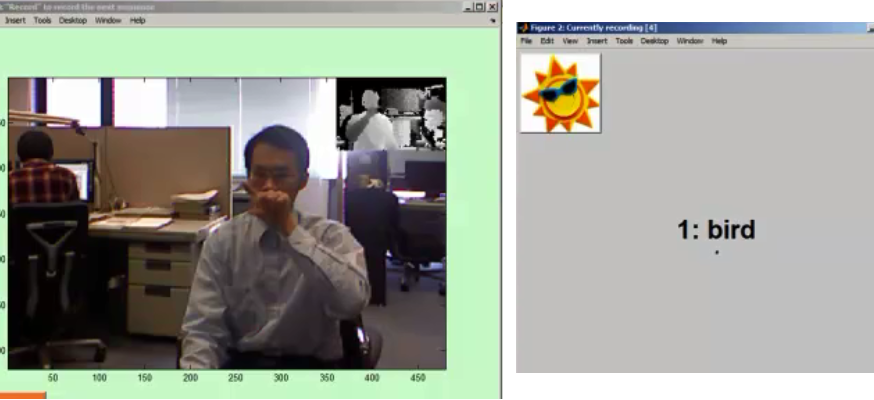
\includegraphics[scale=0.7]{game_demo_2.png}
\caption{Minh họa game tương tác luyện trí nhớ sử dụng ngôn ngữ cử chỉ: Thông báo kết quả cử chỉ thực hiện đã đúng - nghĩa là bộ nhận dạng cử chỉ đã nhận dạng chính xác.}
\label{fig_game_gest_2}
\end{figure}

%\section{Kết chương}

